%% chapter 4 dataset, network structure, experiment and result
\chapter{模型的分析与评估}
\label{cha:experiment}

将验证集中的1000张重建图像输入已训练的模型,得到重建图像的预测图像后,计算预测图象与原图像的MSE、PSNR、SSIM等评价指标,并对比重建图像与原图像之间的MSE、PSNR、SSIM等值,对模型的优化效果进行分析与评估。

\section{MSE}

\subsection{MSE简介}
MSE是衡量两张图片的相似程度的一种常见方法。两个图片之间的MSE即求两张图片各个相对应的像素点的平方差之和的均值。具体公式如下:

\begin{equation} \label{601}
	MSE(I,K)=\cfrac{1}{mn}\sum_{i=0}^{m-1}\sum_{j=0}^{n-1}\big [I(i,j)-K(i,j)]^2
\end{equation}

\subsection{使用MSE衡量模型效果}
计算验证集中的1000张重建图像与原图像的MSE值和预测图像与原图像的MSE值,结果如图\ref{fig601}所示。
 
\begin{figure}[h]
	\centering
	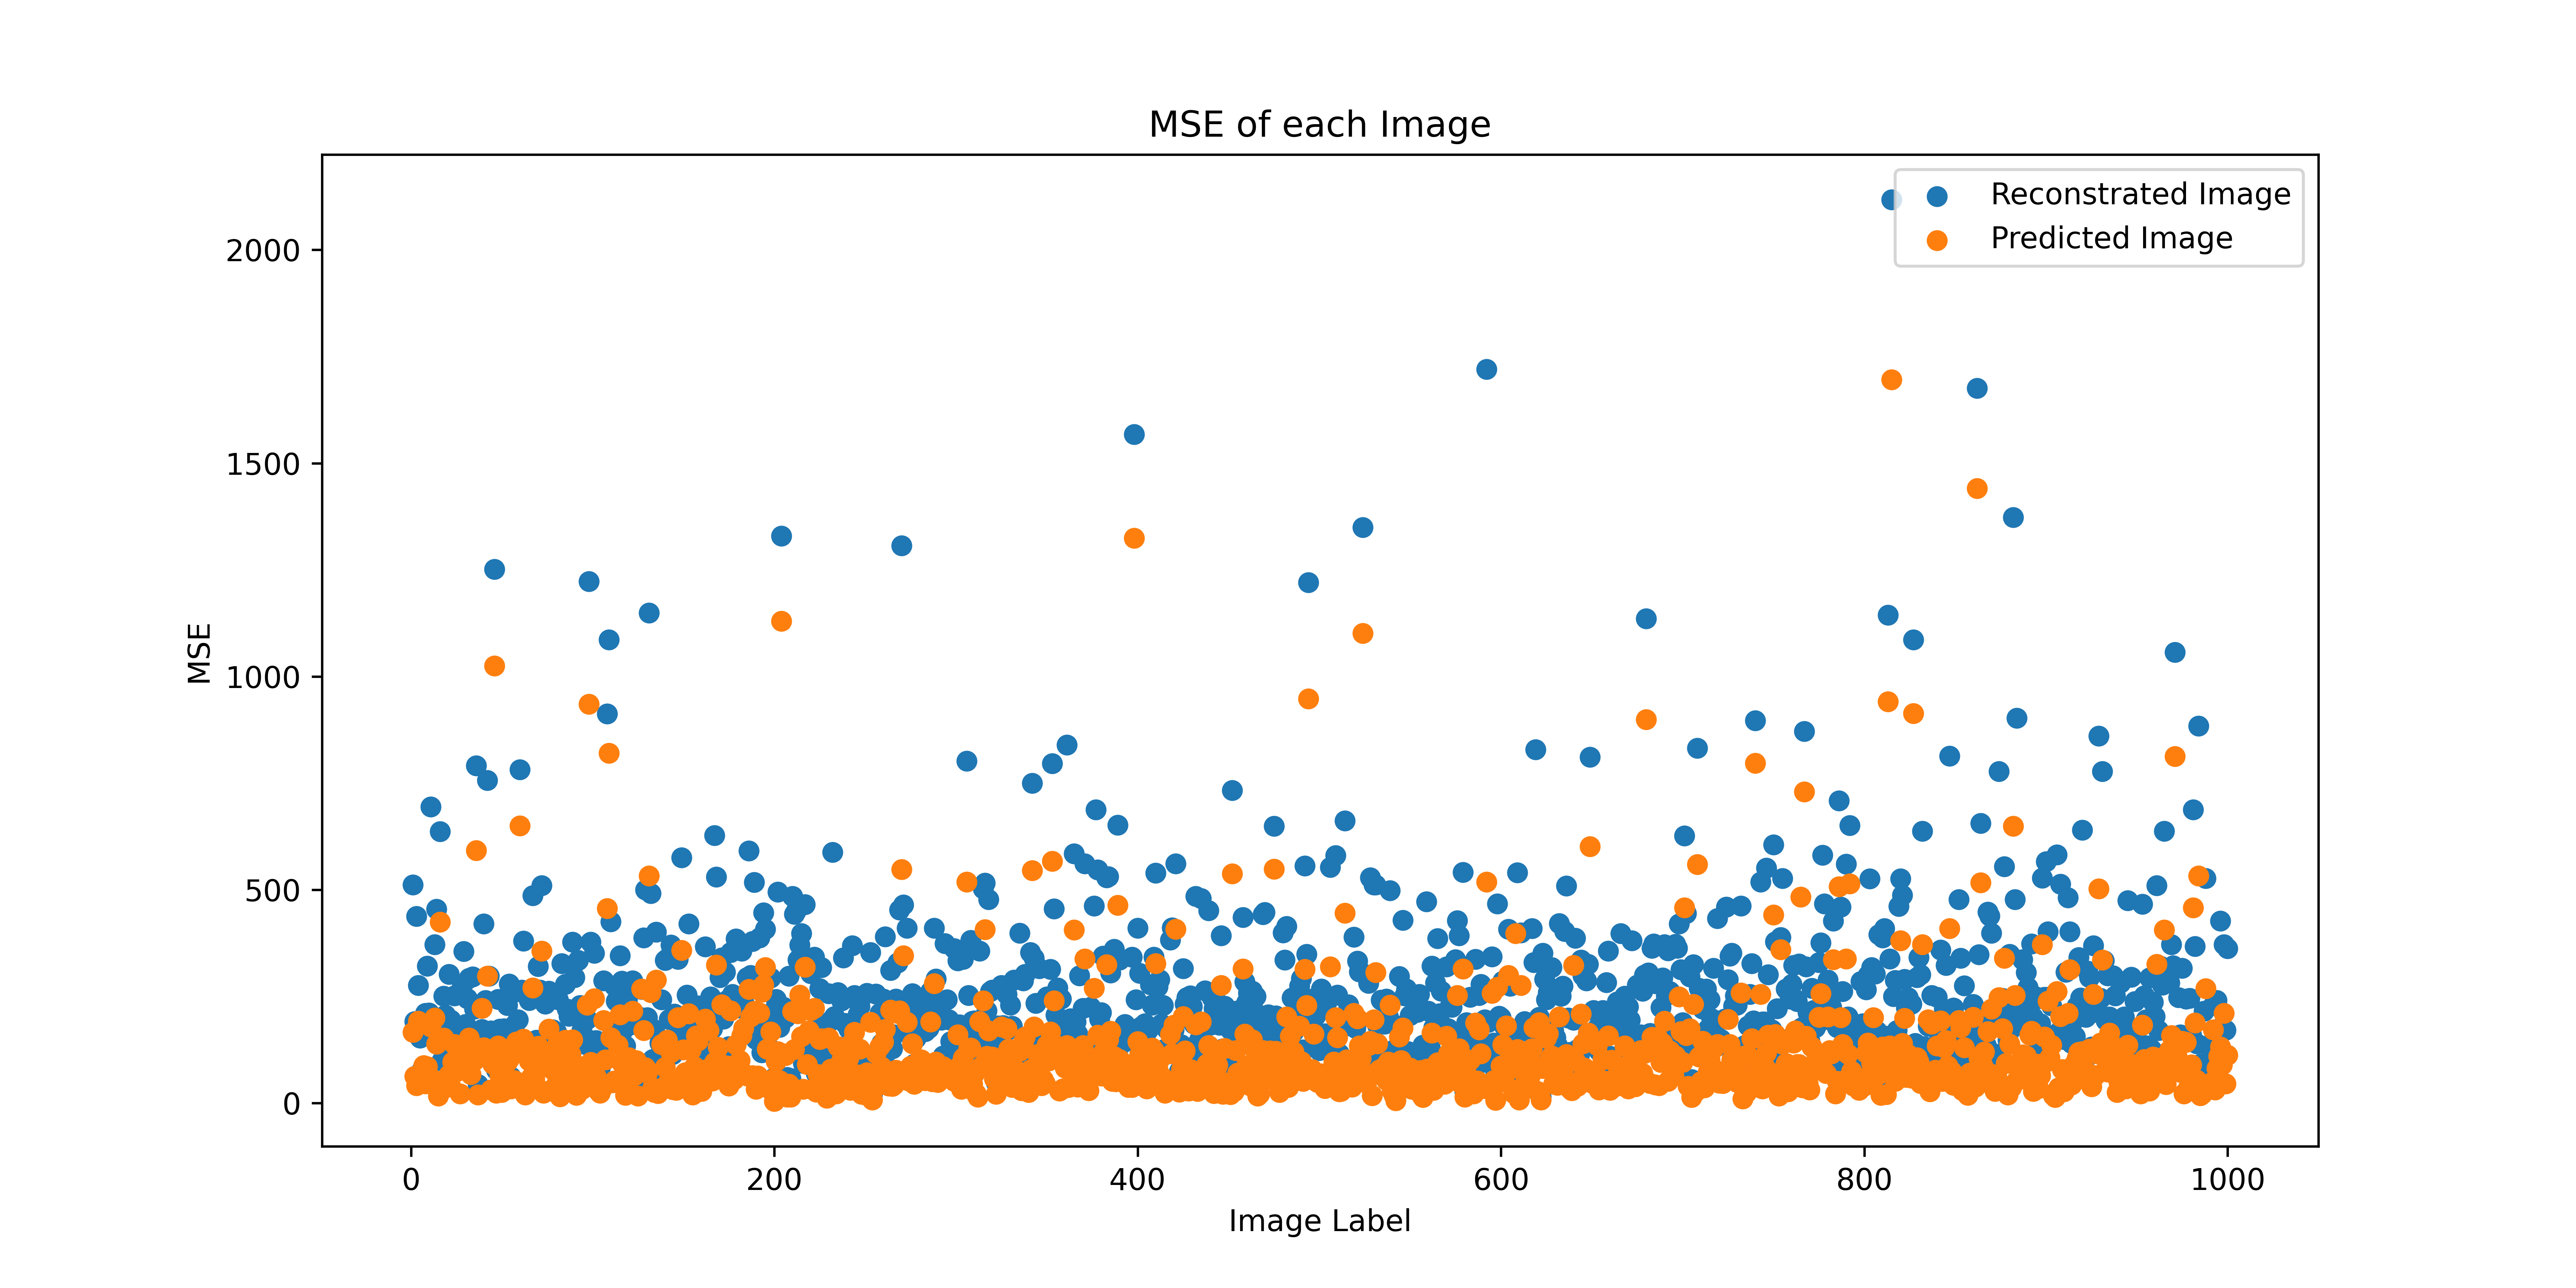
\includegraphics[width=0.9\columnwidth]{image/chap06/img601.png}
	\caption{测试集图像及其预测图象与原图像的MSE}
	\label{fig601}
\end{figure}

在图\ref{fig601}中,X轴为各图像的编号,Y轴为对应的MSE值。从图\ref{fig601}可以看出,预测图象的MSE值在图中的主要分布区域为0到250,而重建图像的MSE值的主要分布区域为100到500。且在MSE值超过500的区域,重建图像的数量显著多于预测图像。进一步,计算这1000张重建图像与预测图像的MSE值的平均值,计算结果如图\ref{fig602}。

\begin{figure}[h]
	\centering
	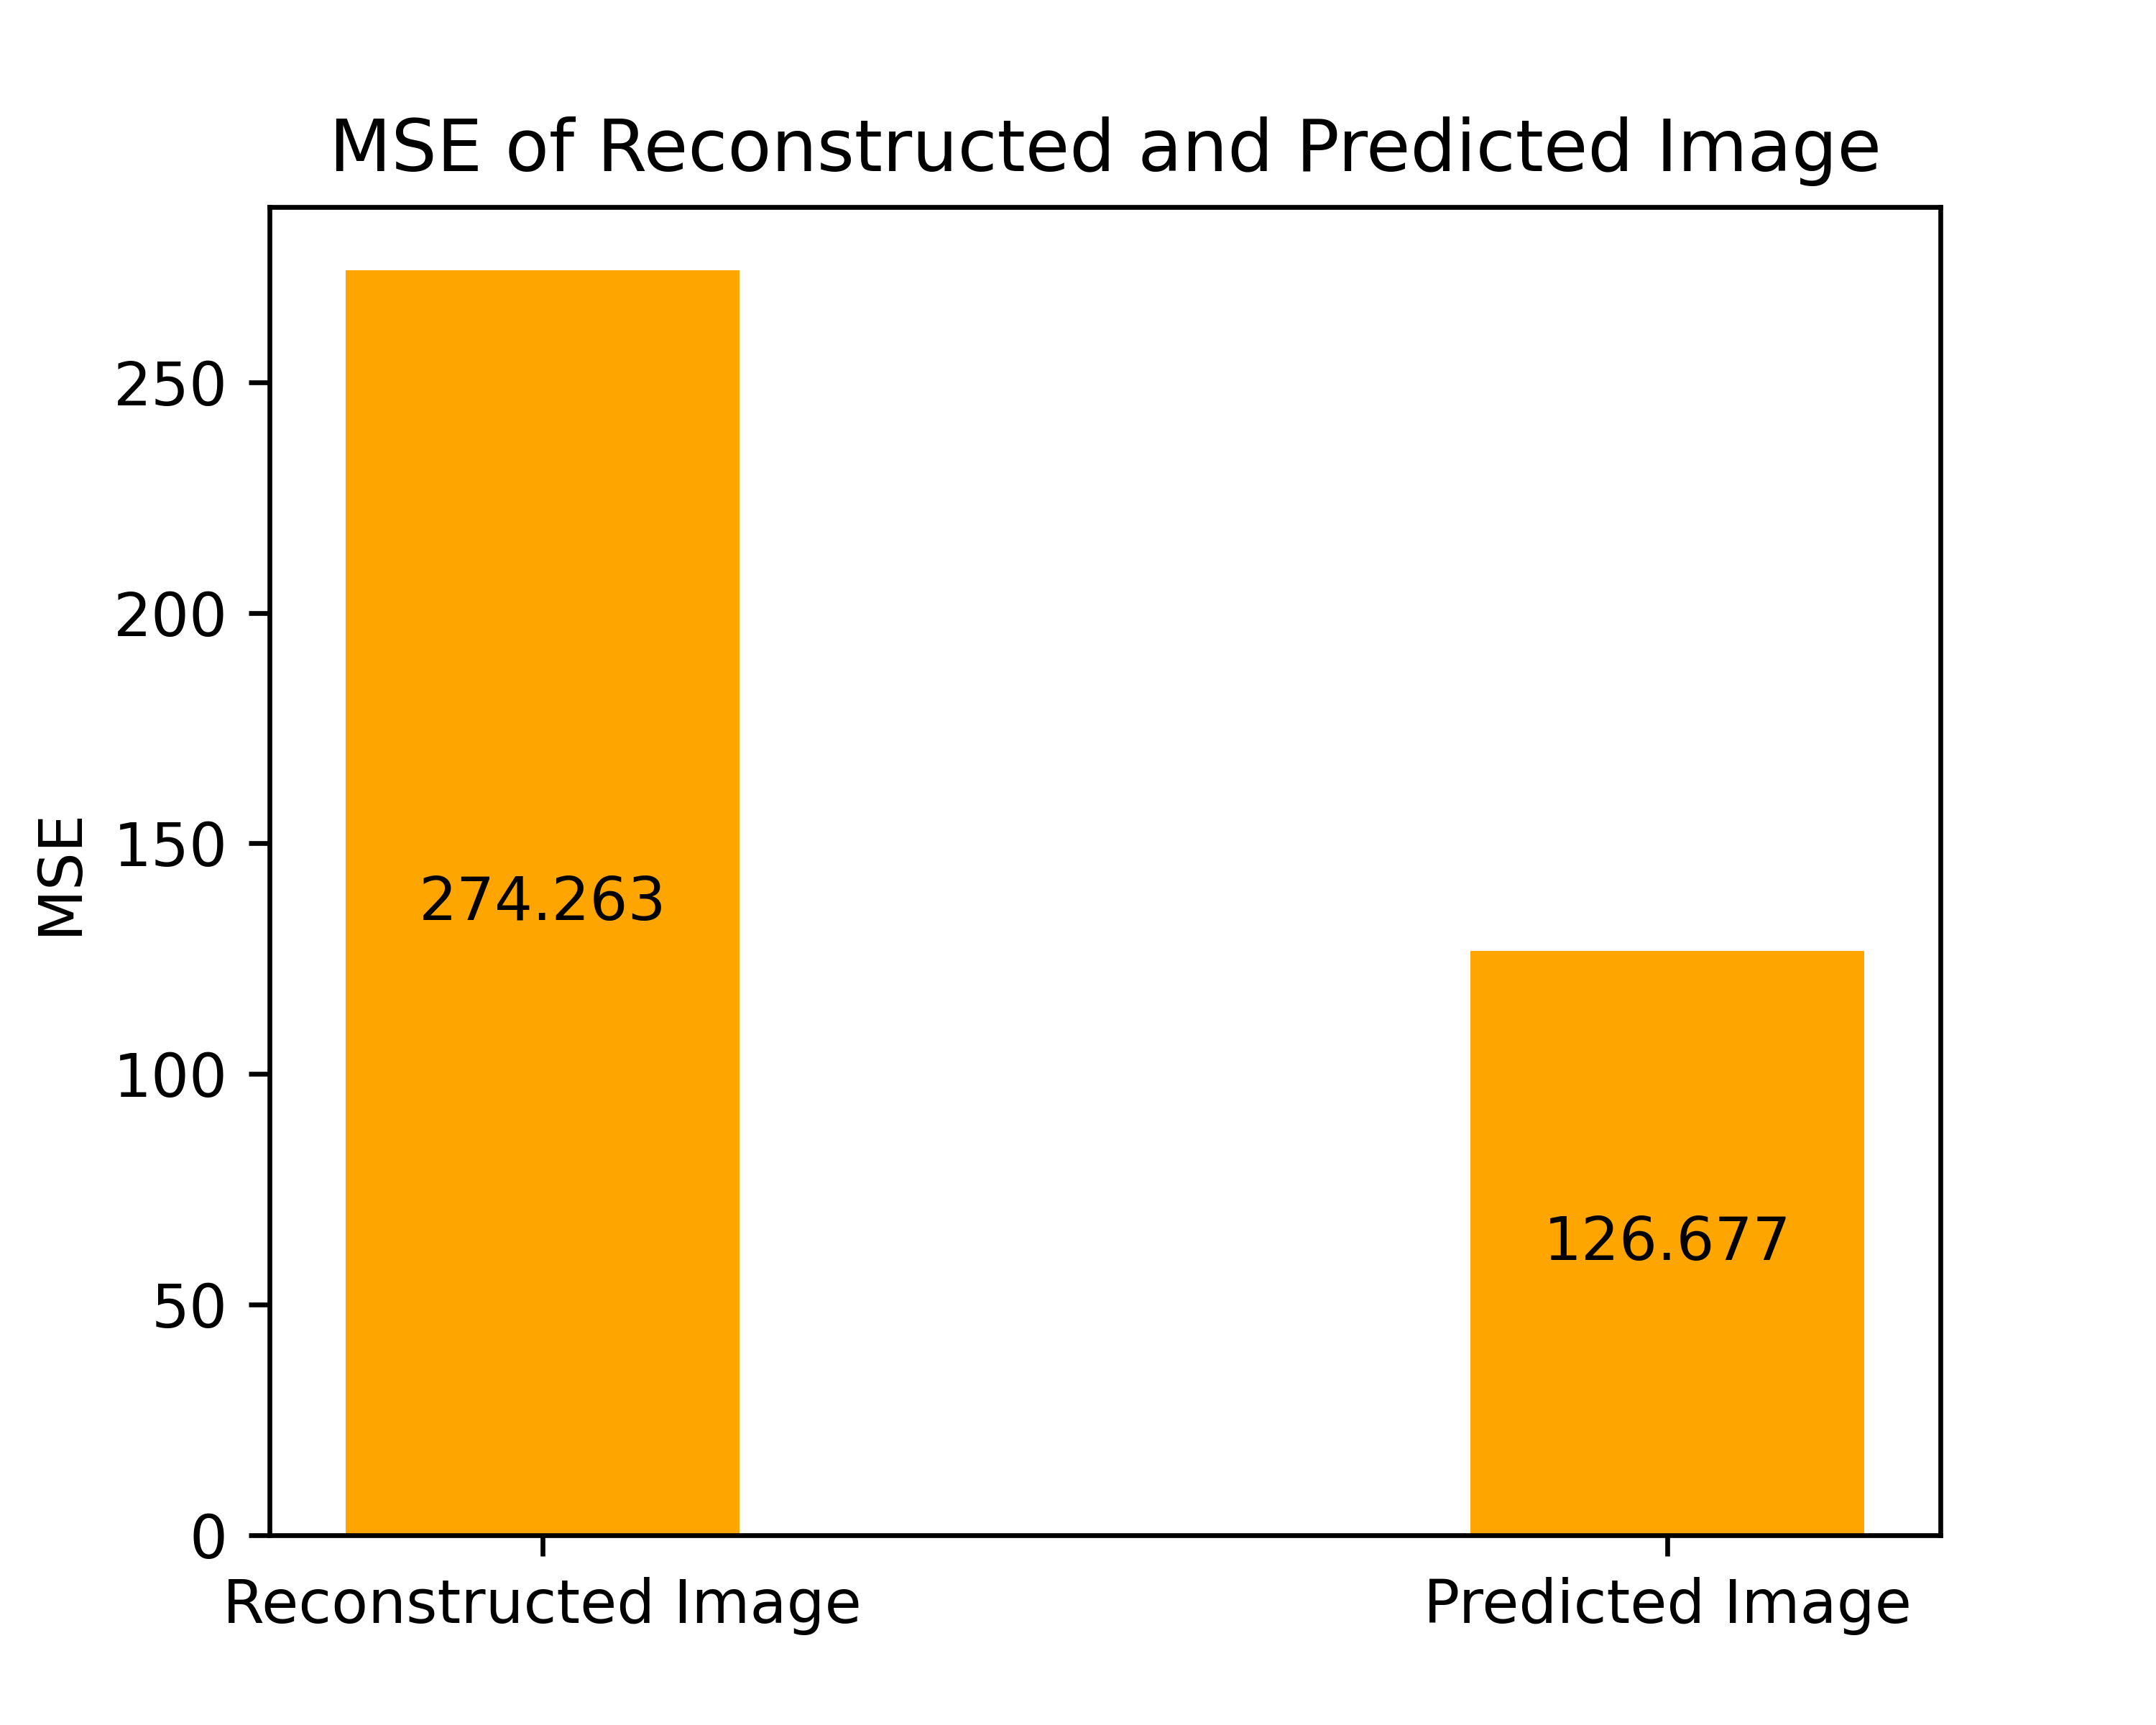
\includegraphics[width=0.75\columnwidth]{image/chap06/img602.png}
	\caption{测试集图像及其预测图象与原图像的MSE的均值}
	\label{fig602}
\end{figure}

 从图\ref{fig602}可以得出,在输入模型后所得优化图像,相比原来的重建图像,平均的MSE值由274.263下降为126.677,这说明模型对原来的重建图像具有良好的优化效果。
 
 \section{PSNR}
 \subsection{PSNR简介}
 PSNR即峰值信噪比,PSNR的计算涉及到MSE。它的公式如下:
 
 \begin{equation} \label{602}
 	\begin{aligned}
 		PSNR(I,K)=10\cdot log_{10}(\cfrac{MAX_I^2}{MSE})
 	\end{aligned}
 \end{equation}

对数内分母为均方误差MSE,分子中的$MAX_I$为最大像素值,即若为b位图像,该值为$2^b-1$。当两张图片的MSE差异越小,则对数内的值越大,此时PSNR就越大。因此,PSNR越大就表示图像相似程度越高。

\subsection{利用PSNR衡量模型效果}
 计算验证集中的1000张重建图像与原图像的PSNR值和预测图像与原图像的PSNR值,结果如图\ref{fig603}所示。
 
 \begin{figure}[h]
 	\centering
 	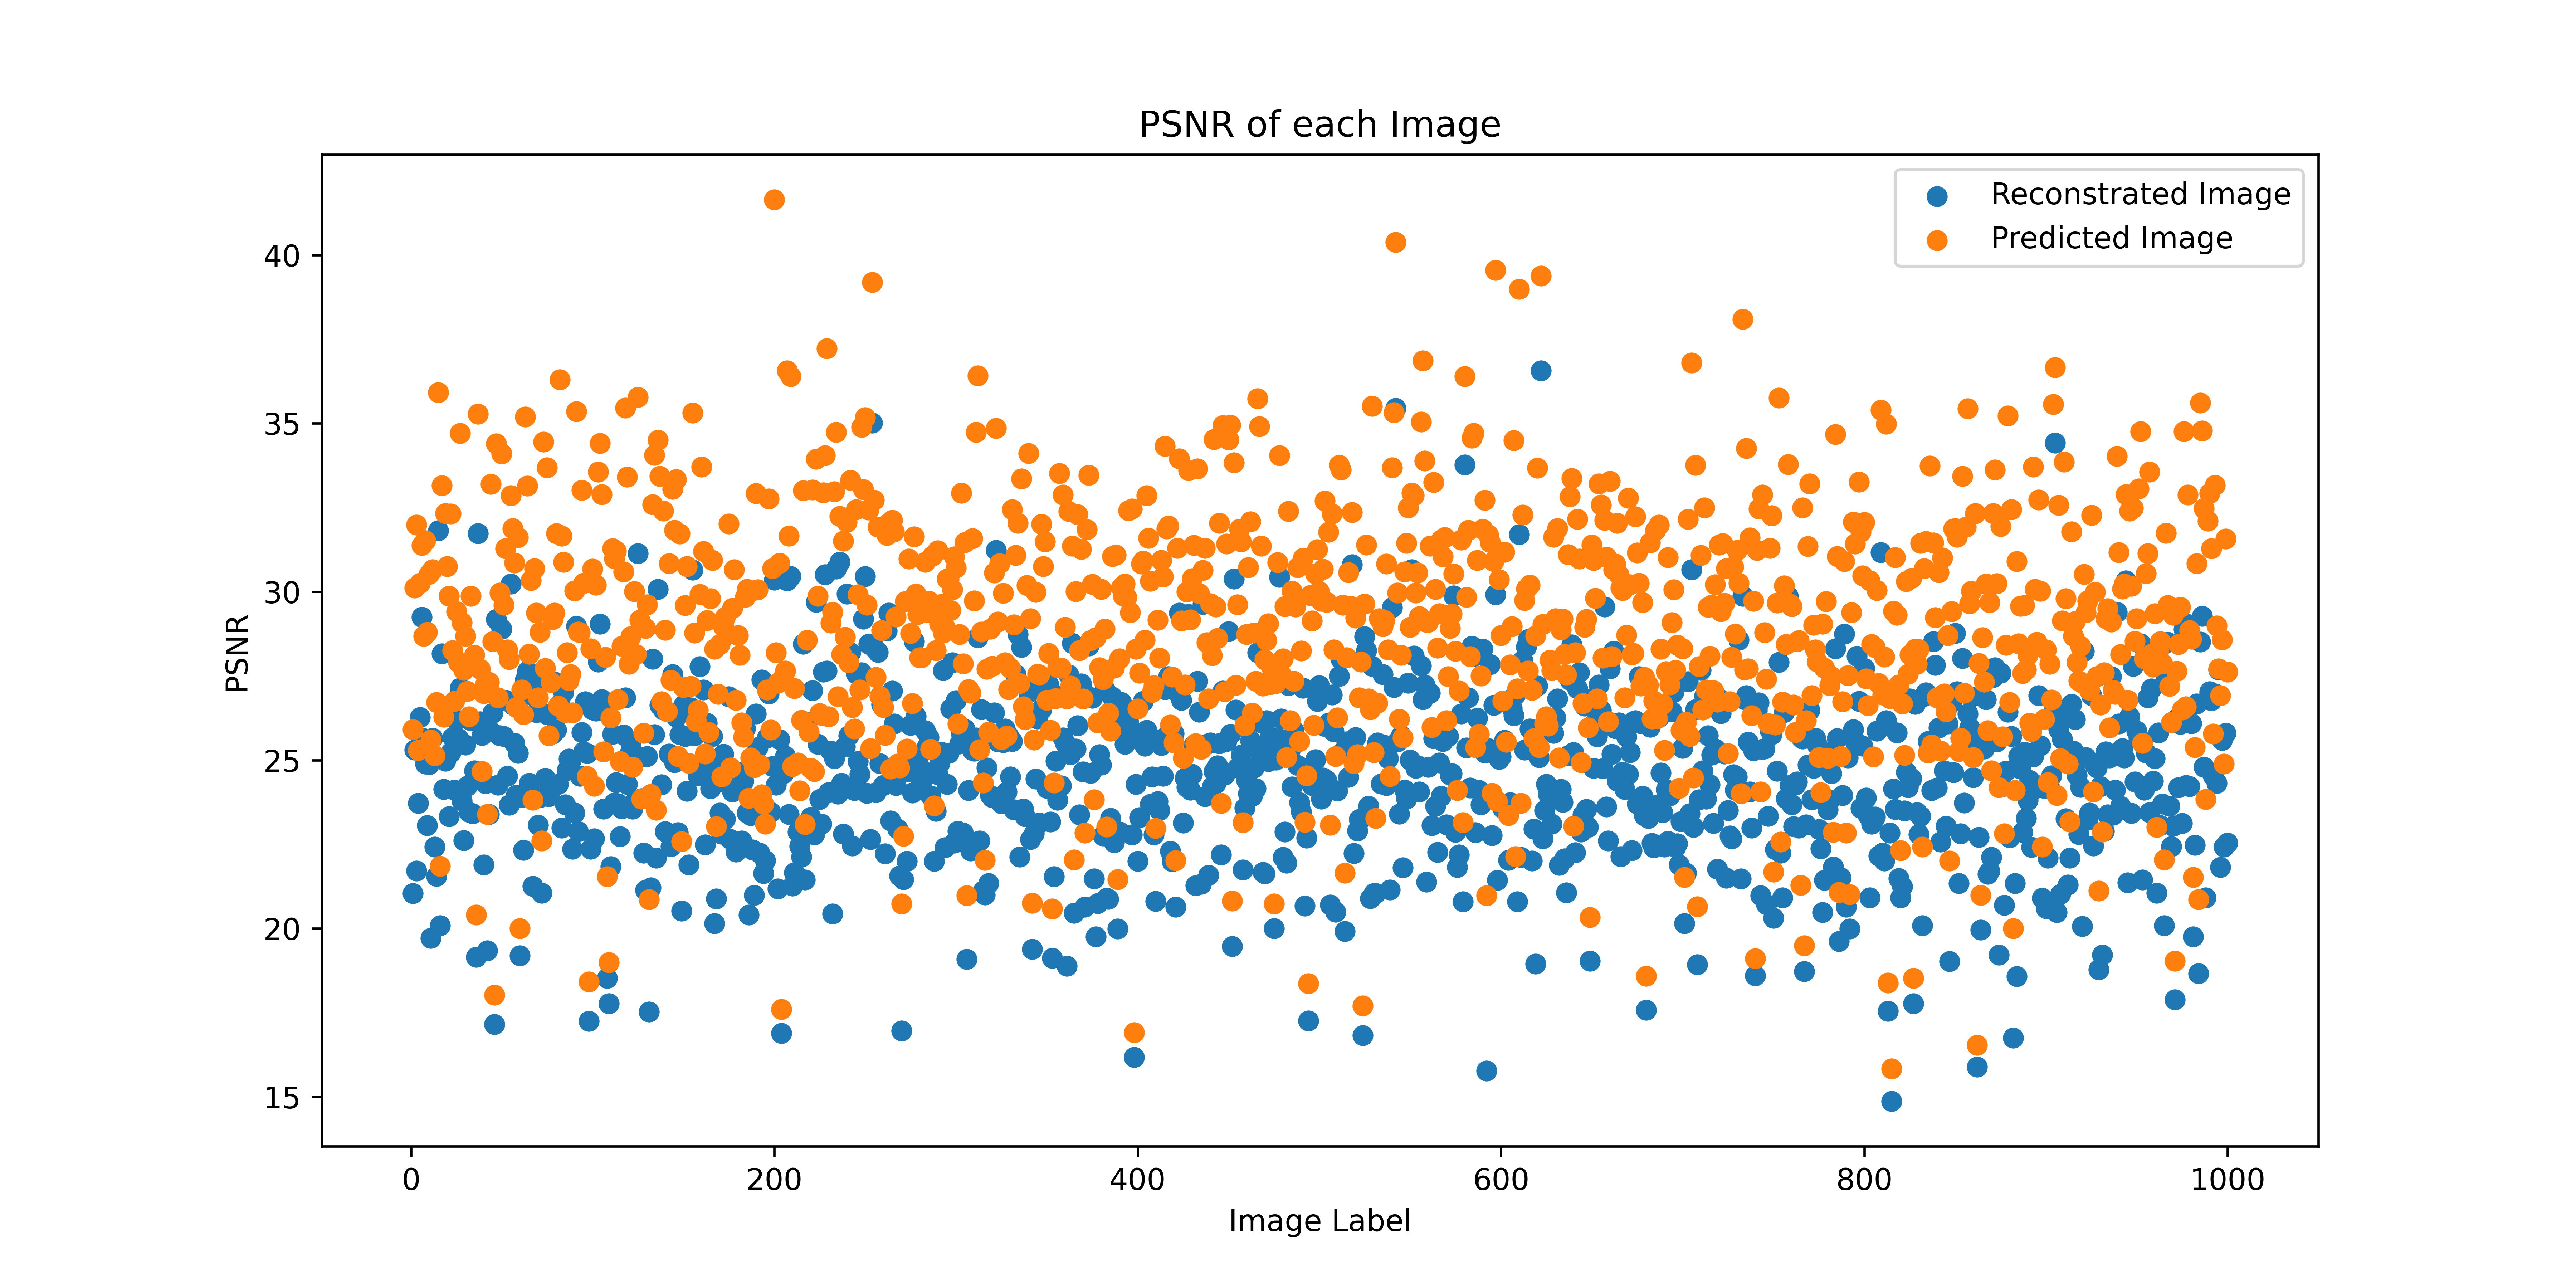
\includegraphics[width=0.9\columnwidth]{image/chap06/img603.png}
 	\caption{测试集图像及其预测图象与原图像的PSNR}
 	\label{fig603}
 \end{figure}

在图\ref{fig603}中,X轴为各图像的编号,Y轴为对应的PSNR值。从图\ref{fig603}可以看出,预测图象的PSNR值在图中的主要分布区域为上半区域,而重建图像的PSNR值主要分布在下半区域。计算这1000张重建图像与预测图像的PSNR值的平均值,计算结果如图\ref{fig604}。

\begin{figure}[h]
	\centering
	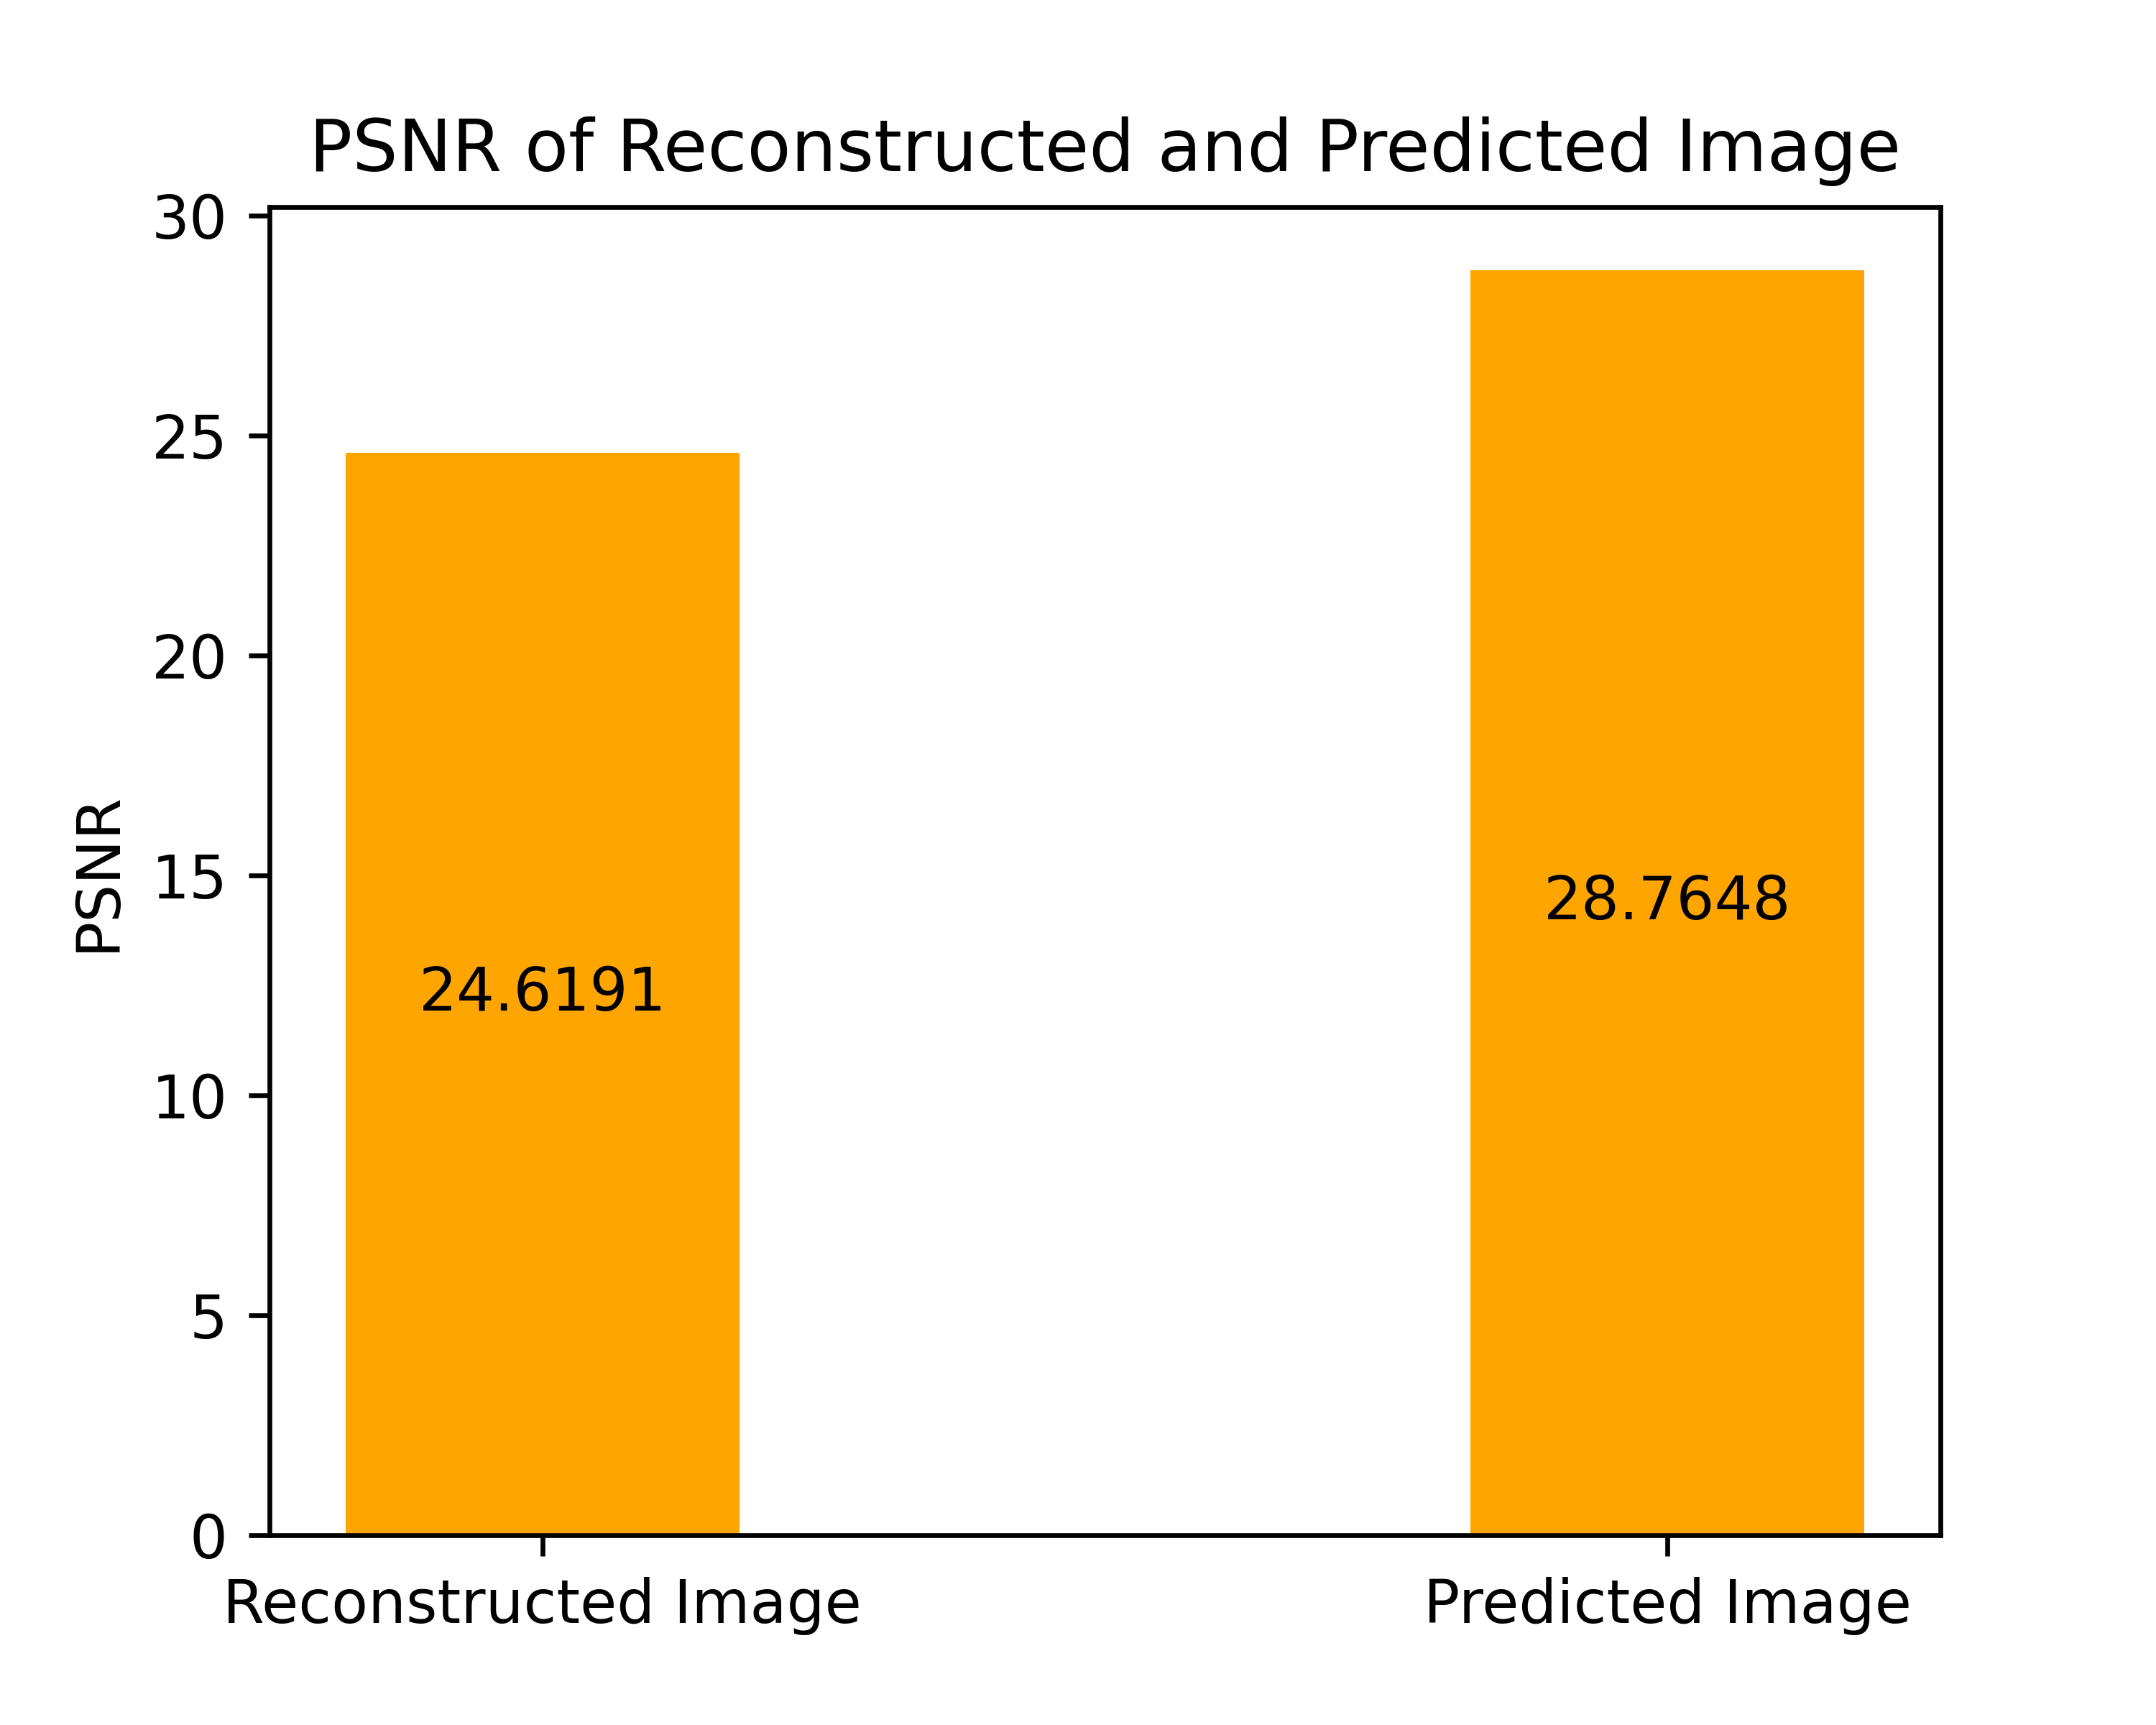
\includegraphics[width=0.75\columnwidth]{image/chap06/img604.png}
	\caption{测试集图像及其预测图象与原图像的PSNR的均值}
	\label{fig604}
\end{figure}

从图\ref{fig604}可以得出,在输入模型后所得优化图像,相比原来的重建图像,平均的PSNR值由24.6191上升为28.7638。由上述PSNR公式可得,更高的PSNR代表着更高的图像相似程度,这说明模型的预测图象相比于重建图像与原图像具有更高的相似度,模型具有良好的优化效果。

\section{SSIM}
\subsection{SSIM简介}
SSIM即结构相似度,它是一种判断两张图片在结构上的差距的一项指标。

与传统的 MSE 不同,对于两张图片基于 MSE 的损失大小不足以表达人类视觉系统对这两张图片所感觉到的差距。比如两张只是亮度不同的图片,由于MSE是计算二者像素差的平方之和,因此所计算出的损失很大,但在人眼看来,这两张图片是十分相近的。人类视觉相关的研究普遍认为人类衡量两幅图的差距,更倾向于比较两图的结构相似性,而不是像MSE那样逐像素计算两图的差异。

SSIM的衡量标准有两张图片的亮度相似度,对比度和结构相似度三个指标。

\subsubsection{亮度相似度}
设图像X所含的像素点个数为N,各像素值为$x_i$,则定义其平均亮度为X中各像素的均值,即:$\mu_X=\cfrac{1}{N}\sum_{i=1}^{N}x_i$

定义衡量两幅图 X 和 Y 的亮度相似度的公式为:

 \begin{equation} \label{603}
	l(X,Y)=\cfrac{2\mu_x\mu_y+C_1}{\mu_x^2+\mu_y^2+C_1}
\end{equation}

其中分母所在的常数是为了后续计算中避免出现分母为 0 的情况。

\subsubsection{对比度}
对比度定义为全体像素值的标准差,代表着图像明暗变化的剧烈程度。一张图像的标准差的计算公式为:
$\sigma_X=\sqrt{\cfrac{\sum_{i=1}^{N}(x_i-\mu_X)^2}{N-1}}$。
衡量两幅图 X 和 Y 的对比度的相似度的公式为:

 \begin{equation} \label{604}
	c(X,Y)=\cfrac{2\sigma_x\sigma_y+C_2}{\sigma_x^2+\sigma_y^2+C_2}
\end{equation}
同样地,分母中的常数是为了后续计算中避免出现分母为0的情况。

\subsubsection{结构相似度}
由于在上面的推导中已考虑亮度和对比度,因此在研究结构相似度时,应该首先排除这两个指标的影响,即将图像进行归一后以排除均值和标准差的影响。定义归一化后的两个向量 $\cfrac{X −\mu_X}{\sigma_X}$和 $\cfrac{Y −\mu_Y}{\sigma_Y}$之间的结构相似度为:

\begin{equation}\label{605}
	\begin{split}
		\ s(X,Y) &= \ \Big (\cfrac{1}{\sqrt{N-1}}\cfrac{X-\mu_X}{\sigma_X} \Big) \cdot \ \Big(\cfrac{1}{\sqrt{N-1}}\cfrac{Y-\mu_Y}{\sigma_Y}\Big)\\
		&= \cfrac{1}{\sigma_X\sigma_Y}\Big (\cfrac{1}{N-1}\sum_{i=1}^N(x_i-\mu_X)(y_i-\mu_Y) \Big )
	\end{split}
\end{equation}

上式中第一行“·”表示向量内积;第二行括号内的部分为协方差公式:$\sigma_{XY}=\cfrac{\sum_{i=1}^N(x_i-\mu_X)(y_i-\mu_Y)}{N-1}$。因此得到结构相似度的表达式为:

\begin{equation}\label{606}
s(X,Y)=\cfrac{\sigma_{XY}+C_3}{\sigma_X\sigma_Y+C_3}
\end{equation}
同理,为了防止后续计算出现分母为 0,分子分母同时加$C_3$。

\subsubsection{得出 SSIM 表达式}
由上面的推导得出的表达式(\ref{603})、(\ref{604})和(\ref{606}),三个标准相乘作为 SSIM 相似度公式,即:

\begin{equation}\label{607}
	SSIM(x,y)=l(x,y)^{\alpha}\cdot c(x,y)^{\beta} \cdot s(x,y)^{\gamma}
\end{equation}

公式中的$\alpha ,\beta ,\gamma$代表上述三个特征在SSIM指标中的占比,当三者都为1时,SSIM的表达式为:

\begin{equation}\label{608}
SSIM(X,Y)=\cfrac{(2\mu_X\mu_Y+C_1)(2\sigma_{XY}+C_2)}{(\mu_X^2+\mu_Y^2+C_1)(\sigma_X^2+\sigma_Y^2+C_2)}
\end{equation}

从以上的推导公式可知,两张图像的SSIM值是一个介于0和1之间的常数,且越接近1代表两张图像越是接近。从这个角度出发,接下来我们将尝试将SSIM作为指标来分析所得模型做出的预测图像的准确程度。

\subsection{使用SSIM衡量模型效果}
计算验证集中的1000张重建图像与原图像的SSIM值和预测图像与原图像的SSIM值,结果如图\ref{fig605}所示。

\begin{figure}[h]
	\centering
	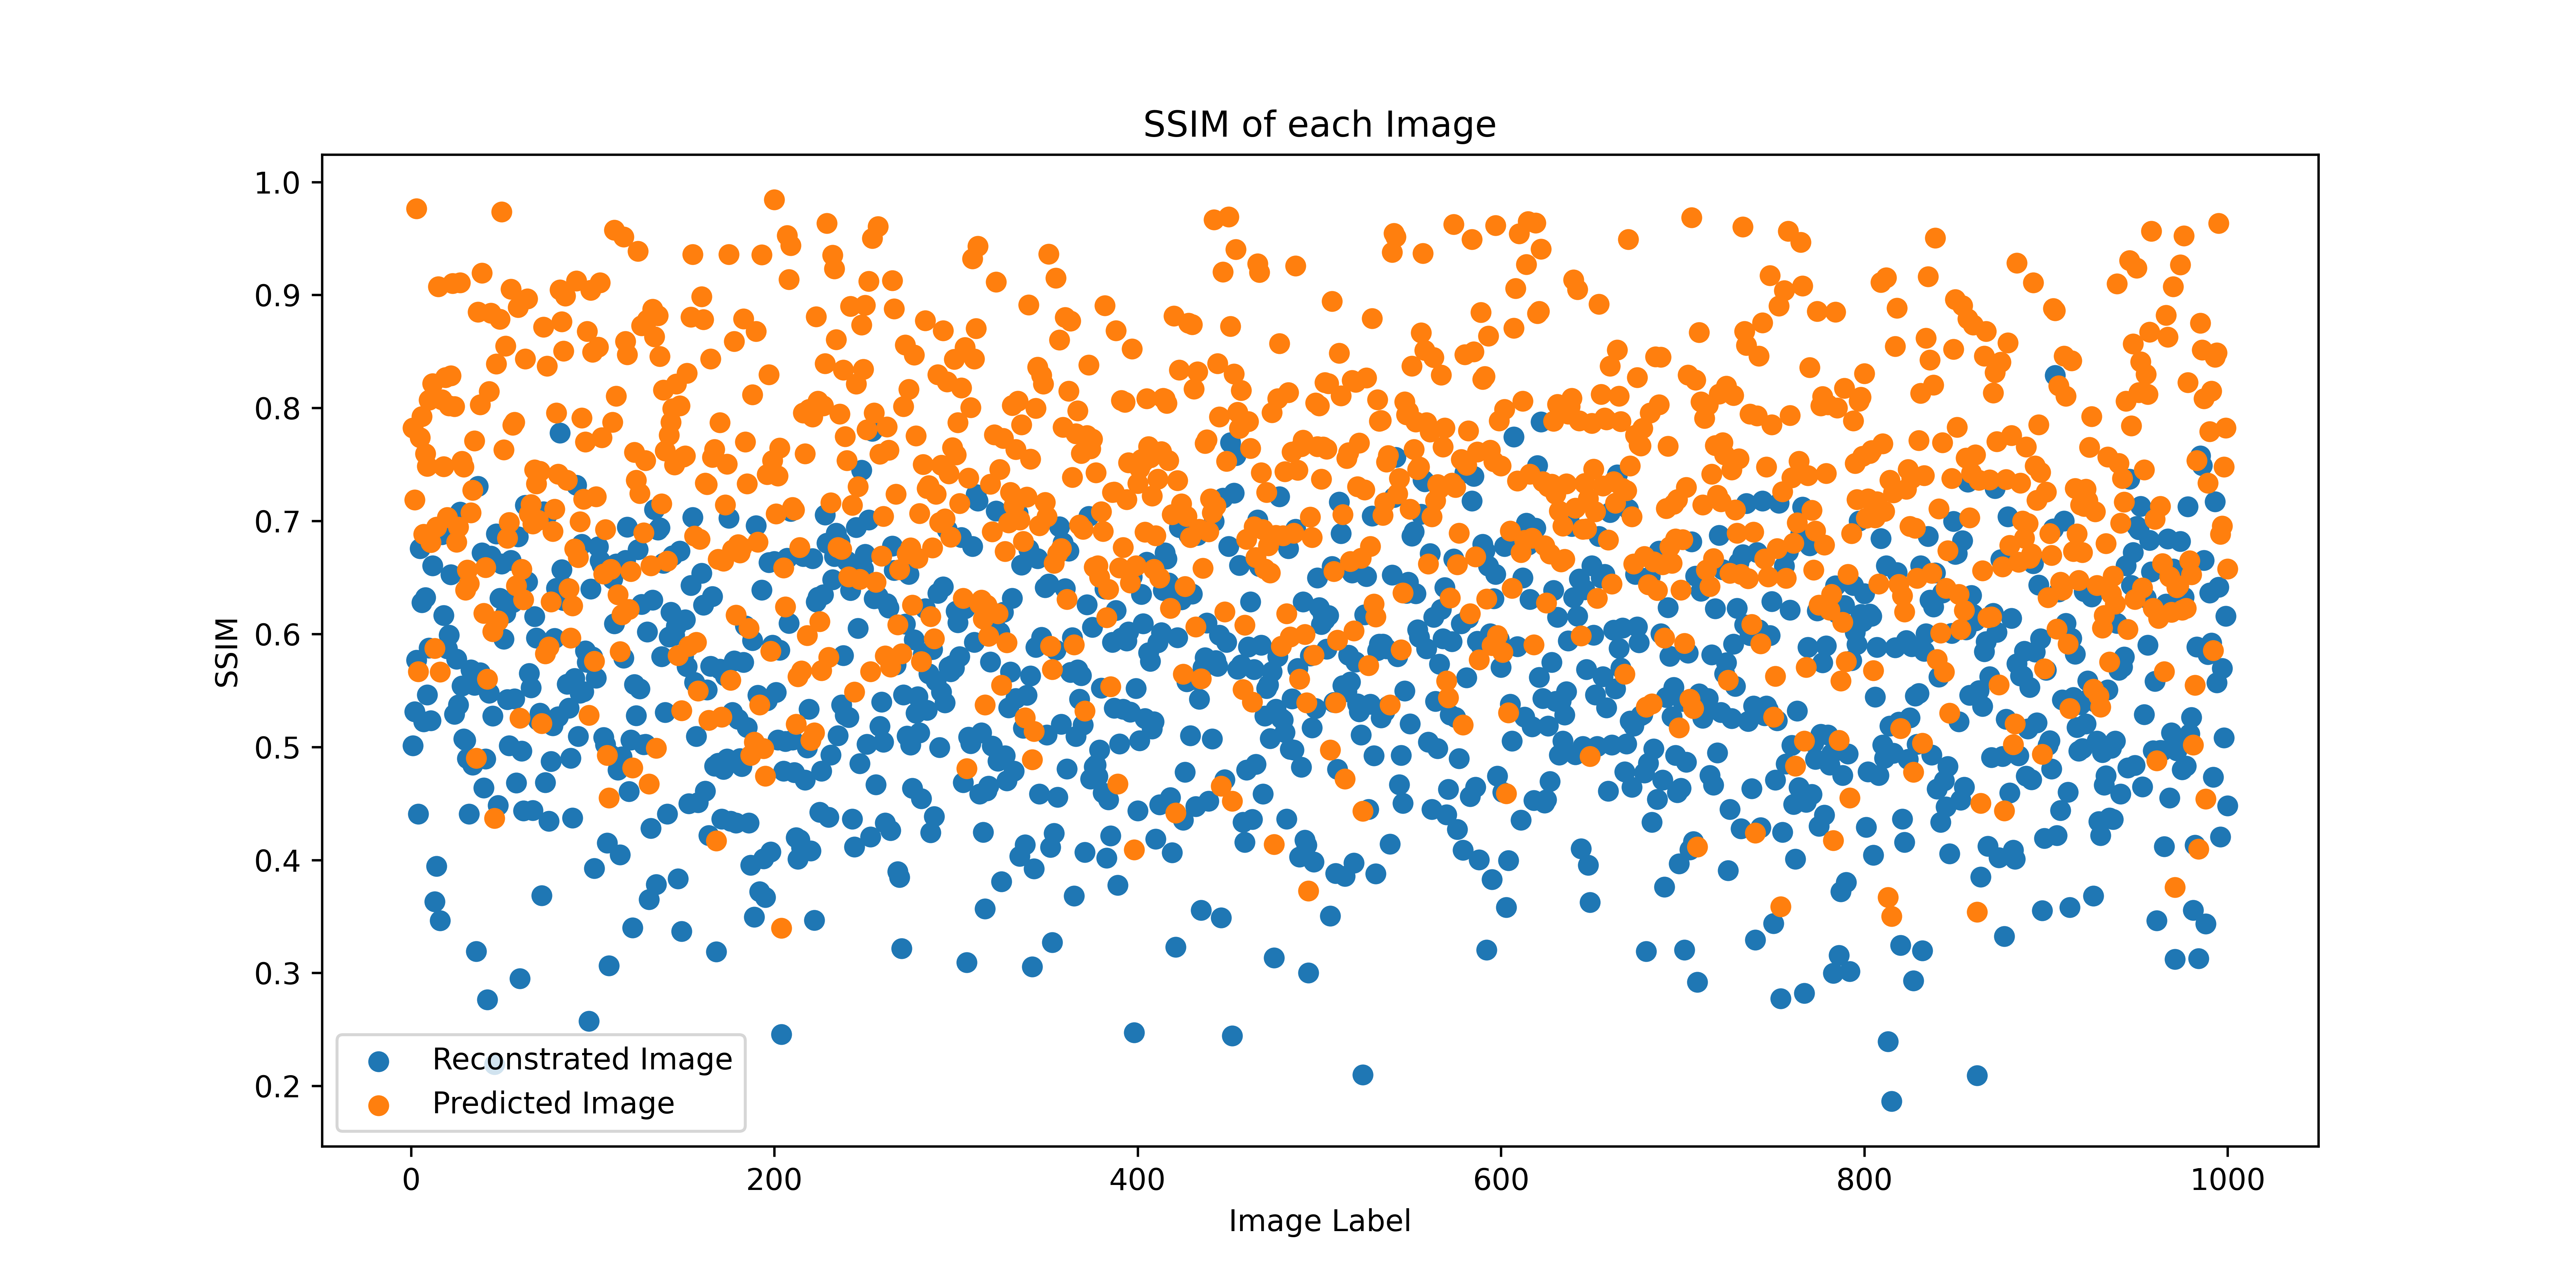
\includegraphics[width=0.9\columnwidth]{image/chap06/img605.png}
	\caption{测试集图像及其预测图象与原图像的SSIM}
	\label{fig605}
\end{figure}

在图\ref{fig605}中,X轴为各图像的编号,Y轴为SSIM值。从图\ref{fig605}可以看出,预测图象的SSIM值在图中大多分布在重建图像的SSIM值之上。而且计算这1000张重建图像与预测图像的SSIM值的平均值,计算结果如图\ref{fig606}。

\begin{figure}[h]
	\centering
	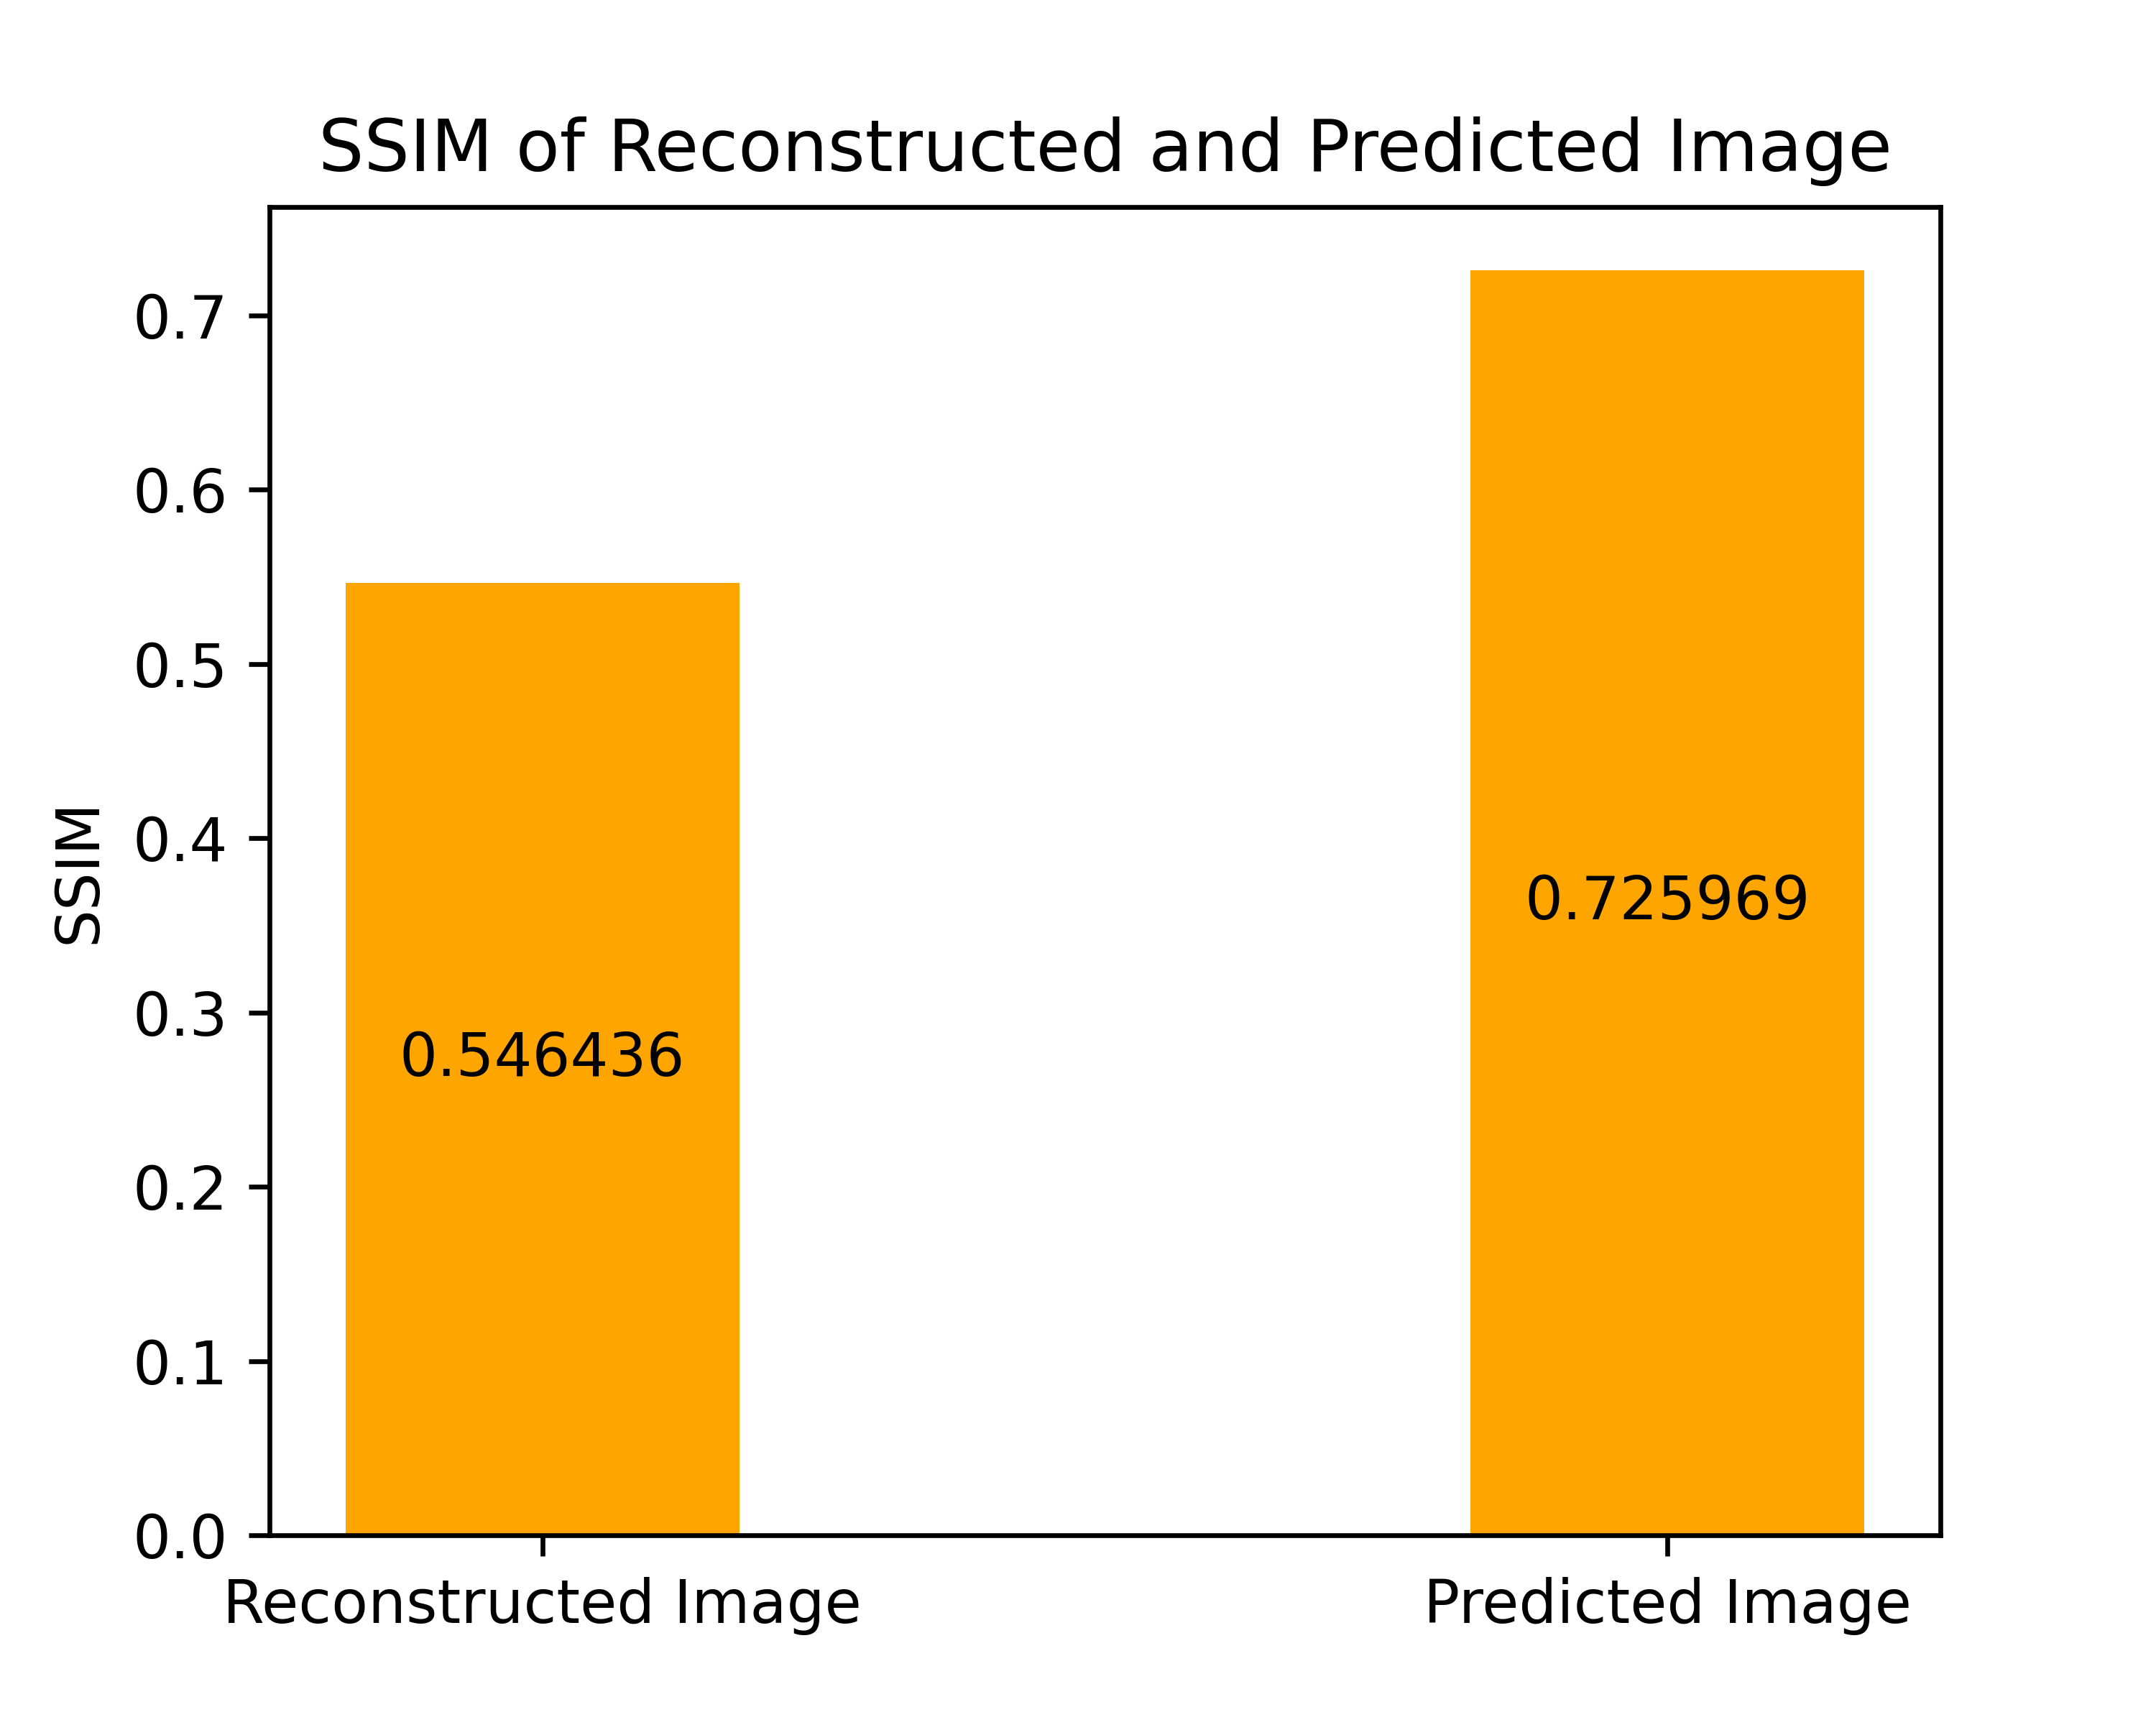
\includegraphics[width=0.75\columnwidth]{image/chap06/img606.png}
	\caption{测试集图像及其预测图象与原图像的SSIM的均值}
	\label{fig606}
\end{figure}

从图\ref{fig606}可以得出,在输入模型后所得优化图像,相比原来的重建图像,平均的SSIM值由0.55上升为0.73。可以发现预测图像对应的 SSIM 值比较接近 1,这说明从 SSIM 的角度上看,原图像与预测出的图像在亮度、对比度与结构相似度上较为接近,所以该模型的预测还是较为准确的。

\section{余弦相似度}
\subsection{余弦相似度简介}

余弦相似度是衡量两个向量相似程度的一项指标,即使用两个向量之间的夹角的余弦值作为衡量两者相似程度的标准。余弦值越接近于1,表示夹角越接近于0,表明两者越相似;反之,余弦值越接近于0,表示夹角约接近于$\cfrac{\pi}{2} $,表明两者越不相似。对于两个向量$X={x_i}$和$Y={y_i}$而言,其余弦相似度的计算公式为:

\begin{equation}\label{609}
	Cosine\ Similarity(X,Y)=\cfrac{\sum_{i=1}^n(x_i\times y_i)}{\sqrt{\sum_{i=1}^n(x_i)^2}\times \sqrt{\sum_{i=1}^n(y_i)^2}}
\end{equation}
我们可以将两张图片表示为向量后,使用余弦相似度来衡量两张图片的相似程度。

\subsection{使用余弦相似度衡量模型效果}
对验证集的1000张图像,我们计算了原图像与重建图像或预测图像间的余弦相似度,将其结果画成直方图如图\ref{fig607}所示。

\begin{figure}[h]
	\centering
	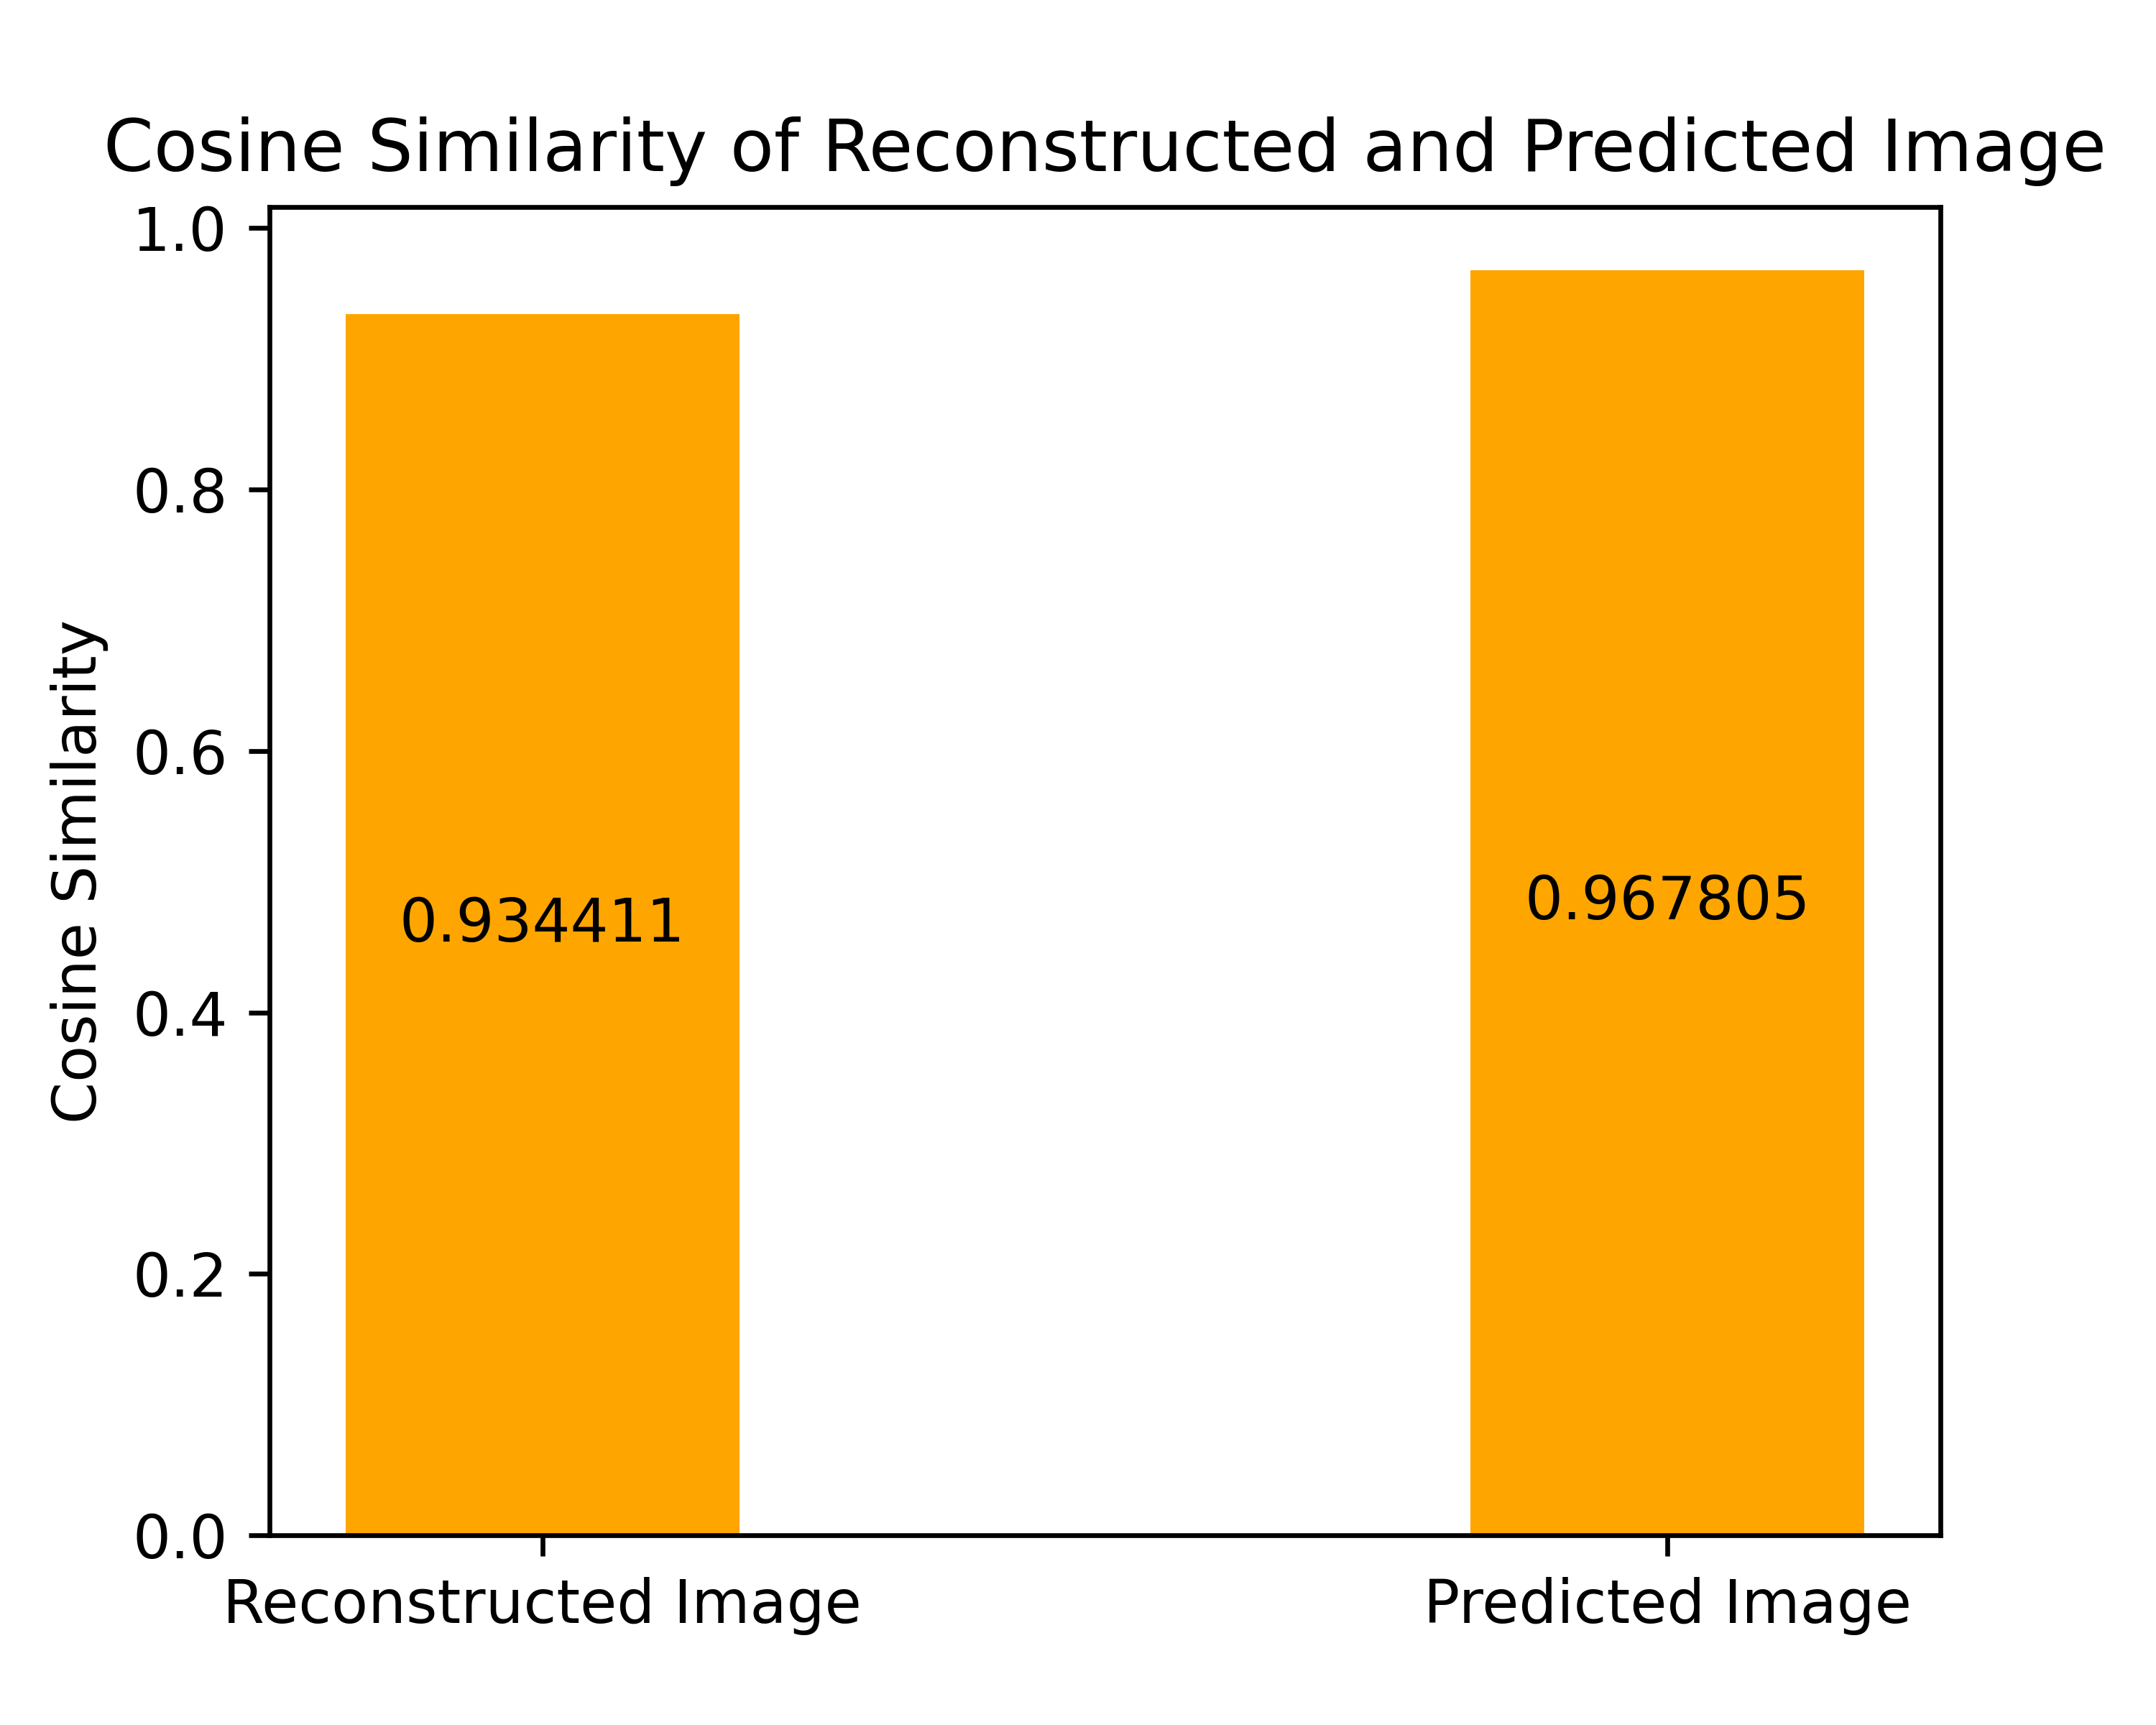
\includegraphics[width=0.75\columnwidth]{image/chap06/img607.png}
	\caption{测试集图像及其预测图象与原图像的余弦相似度的均值}
	\label{fig607}
\end{figure}

从上述结果可以看出,预测图像与原图像的余弦相似度大于重建图像与原图像间的余弦相似度,这说明在余弦相似度的指标下,预测图象对比重建图像具有更高的相似程度。

\section{哈希相似度}
\subsection{哈希相似度简介}
使用哈希值衡量两张图片的相似度分三步:第一步,计算两张图片各自的哈希值;第二步,计算两个哈希值之间的汉明距离(Hamming Distance);第三步,将汉明距离转化为两张图片的相似度。
\subsubsection{计算哈希值}
哈希值有三种定义方法,它们分别是均值哈希值(aHash),差值哈希值(dHash),感知哈希值(pHash)。它们的计算方法如下:
\begin{itemize}
	\item [1)]
	均值哈希值
	\begin{itemize}
		\item [$\bullet$]将图像缩放成如8x8像素大小的小图像并转为灰度图,计算小图像像素的均值。
		\item [$\bullet$]将小图像中比均值高的像素转换为1,比均值小的像素转换为0,生成哈希码。
	\end{itemize}
	
	\item [2)]
	差值哈希值
	\begin{itemize}
		\item [$\bullet$]将图像缩放成8x9像素大小的小图像并转为灰度图,使得每行9个像素之间存在8个不同的差异值。
		\item [$\bullet$]对于小图像中的相邻像素,若左像素比其右像素的值大,则左像素转换为1;否则转换为0,最终得到一个8x8的哈希矩阵。
	\end{itemize}

	\item [3)]
	感知哈希值
	\begin{itemize}
		\item [$\bullet$]将图像缩放成如8x8像素大小的小图像并转为灰度图
		\item [$\bullet$]对小图像进行32x32的DCT(离散余弦变换)得到32x32的DCT系数矩阵,并取左上角的8x8的矩阵,计算该矩阵的平均值。
		\item [$\bullet$]将8x8矩阵中比均值高的元素转换为1,比均值小的元素转换为0,生成哈希码。
	\end{itemize}
	
\end{itemize}

\subsubsection{计算汉明距离}
汉明距离即两个哈希值之间不相等的元素个数。

\subsubsection{将汉明距离转化为两张图片的相似度}
转化为相似度的公式为:

\begin{equation}\label{610}
similarity = 1 - \cfrac{dist}{pixelnum}
\end{equation}
其中dist为汉明距离,pixelnum为小图像的像素个数(若小图像为8x8,则pixelnum等于64)

\subsection{使用哈希相似度衡量模型效果}
对验证集的1000张图像,我们计算了原图像与重建图像或预测图像间的三种哈希相似度,将其结果画成直方图如图\ref{fig608}所示。

\begin{figure}[h]
	\centering
	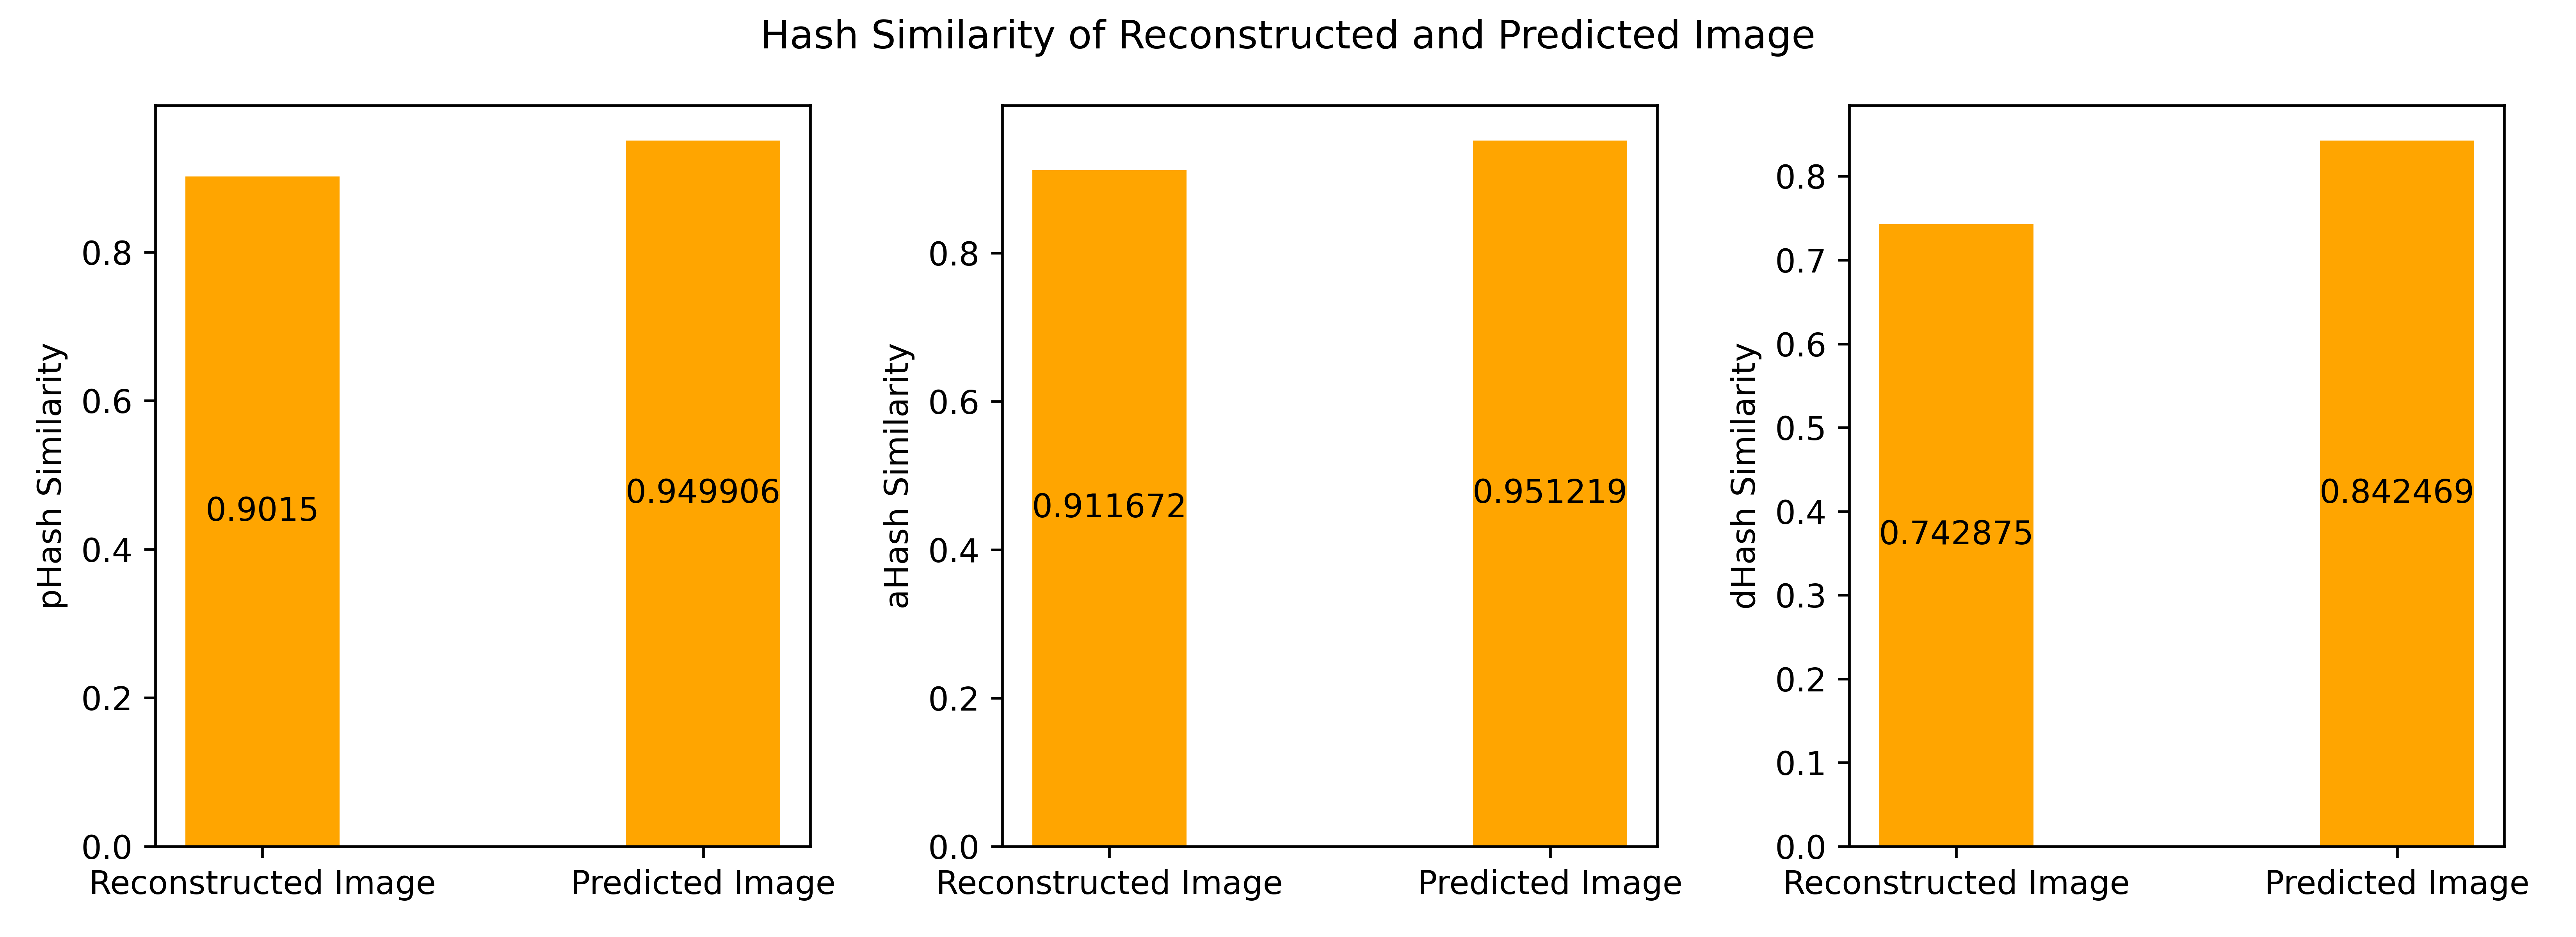
\includegraphics[width=0.9\columnwidth]{image/chap06/img608.png}
	\caption{测试集图像及其预测图象与原图像的三种哈希相似度的均值}
	\label{fig608}
\end{figure}

从图\ref{fig608}可得,无论是均值哈希值,差值哈希值还是感知哈希值,预测图像的相似度均大于重建图像的相似度。

\section{直方图相似度}
\subsection{直方图简介}
图像的直方图即统计全图各像素值所占的像素个数的直方图。对于256值的灰度图而言,就是统计0$ \sim $255这256个值的像素个数所作而成的直方图。例如皮肤癌数据集图像的直方图见图\ref{fig609}。

\begin{figure}[h]
	\centering
	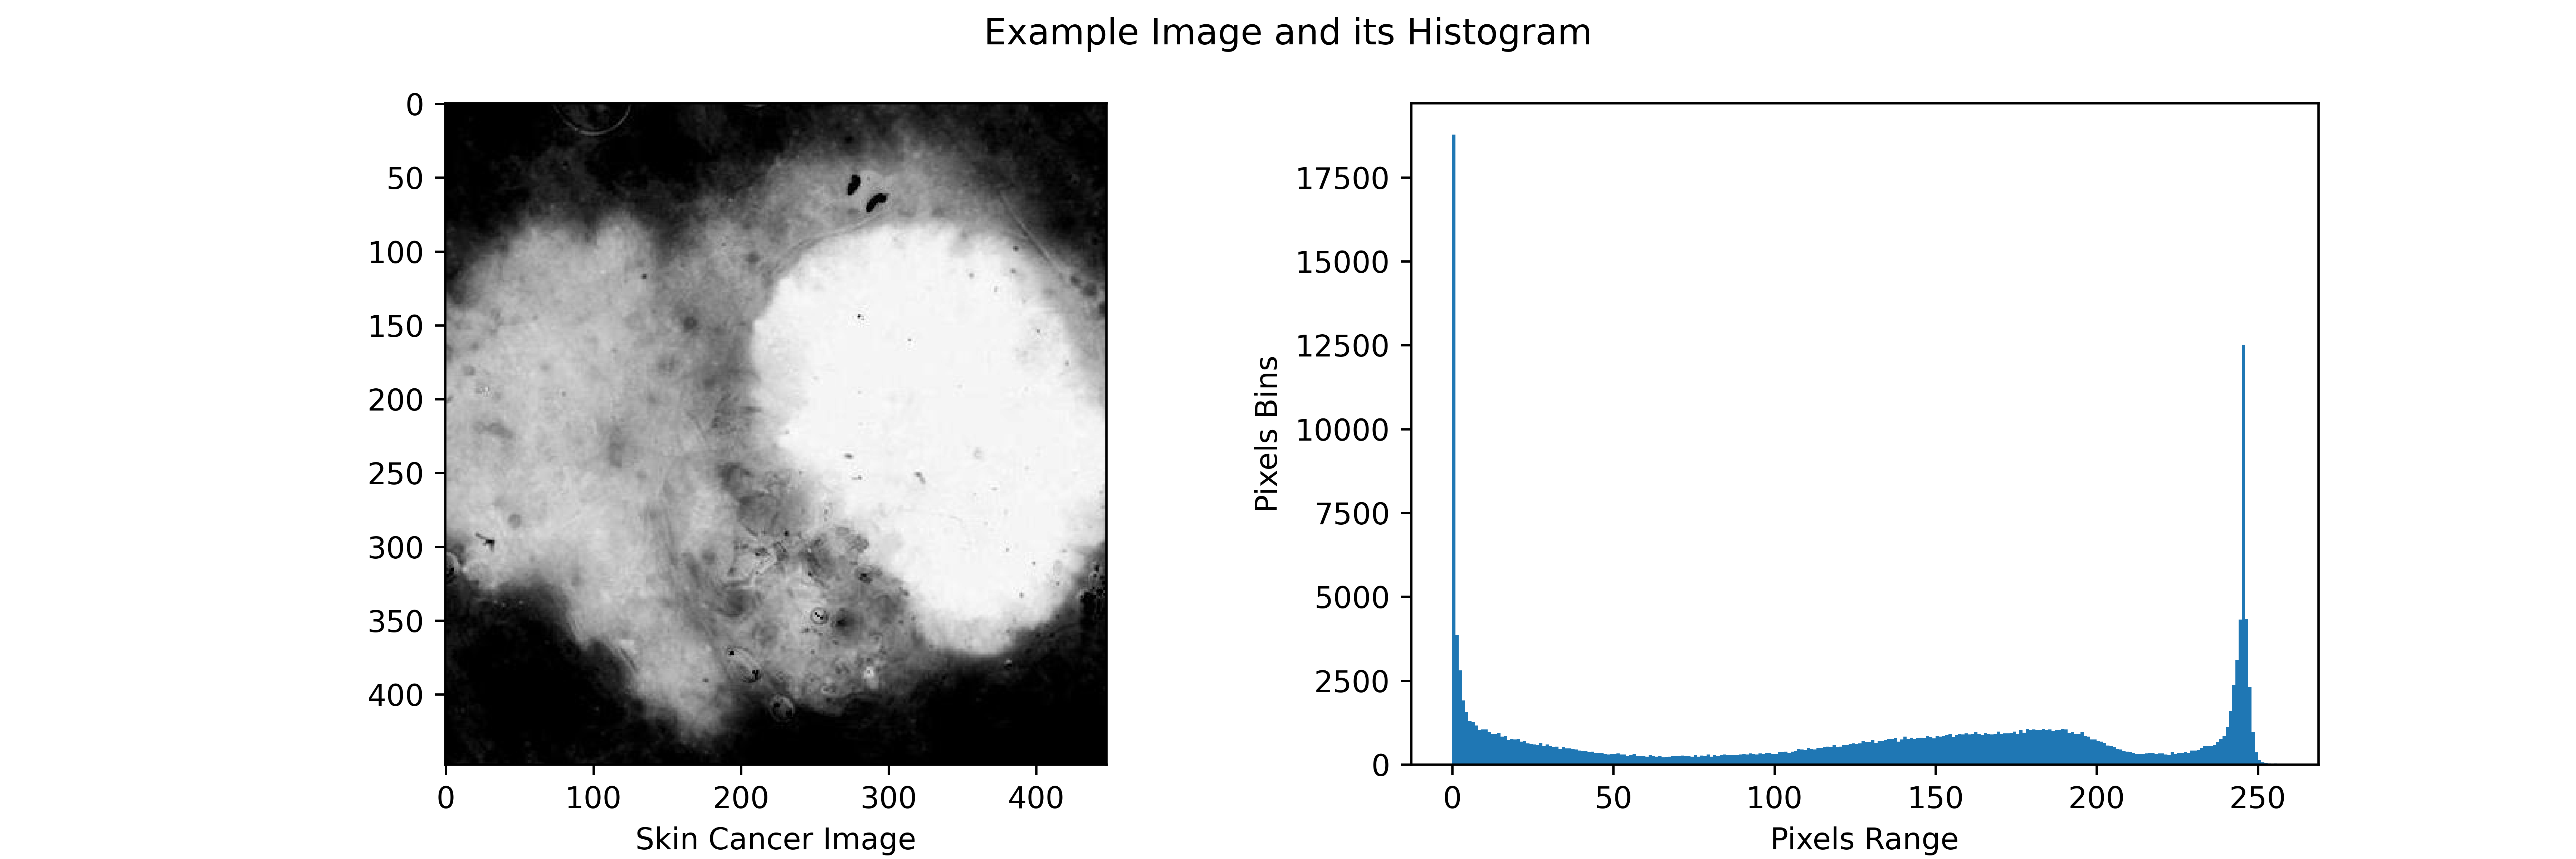
\includegraphics[width=0.9\columnwidth]{image/chap06/img609.png}
	\caption{皮肤癌图片的直方图}
	\label{fig609}
\end{figure}

\hspace*{\fill} \

\hspace*{\fill} \

\hspace*{\fill} \

\hspace*{\fill} \

假设$hist_1$和$hist_2$是存放着0$ \sim $255像素值所占像素个数的数组,则两个图像间的直方图相似度的计算公式为:

\begin{equation}\label{609}
	Degree(hist_1,hist_2)=\sum_i\cfrac{1 - |hist_1[i] - hist_2[i]|}{max(hist_1[i],hist_2[i])}
\end{equation}

\subsection{使用直方图相似度衡量模型效果}
对验证集的1000张图像,我们计算了原图像与重建图像或预测图像间的直方图相似度,其结果如图\ref{fig610}所示。

\begin{figure}[h]
	\centering
	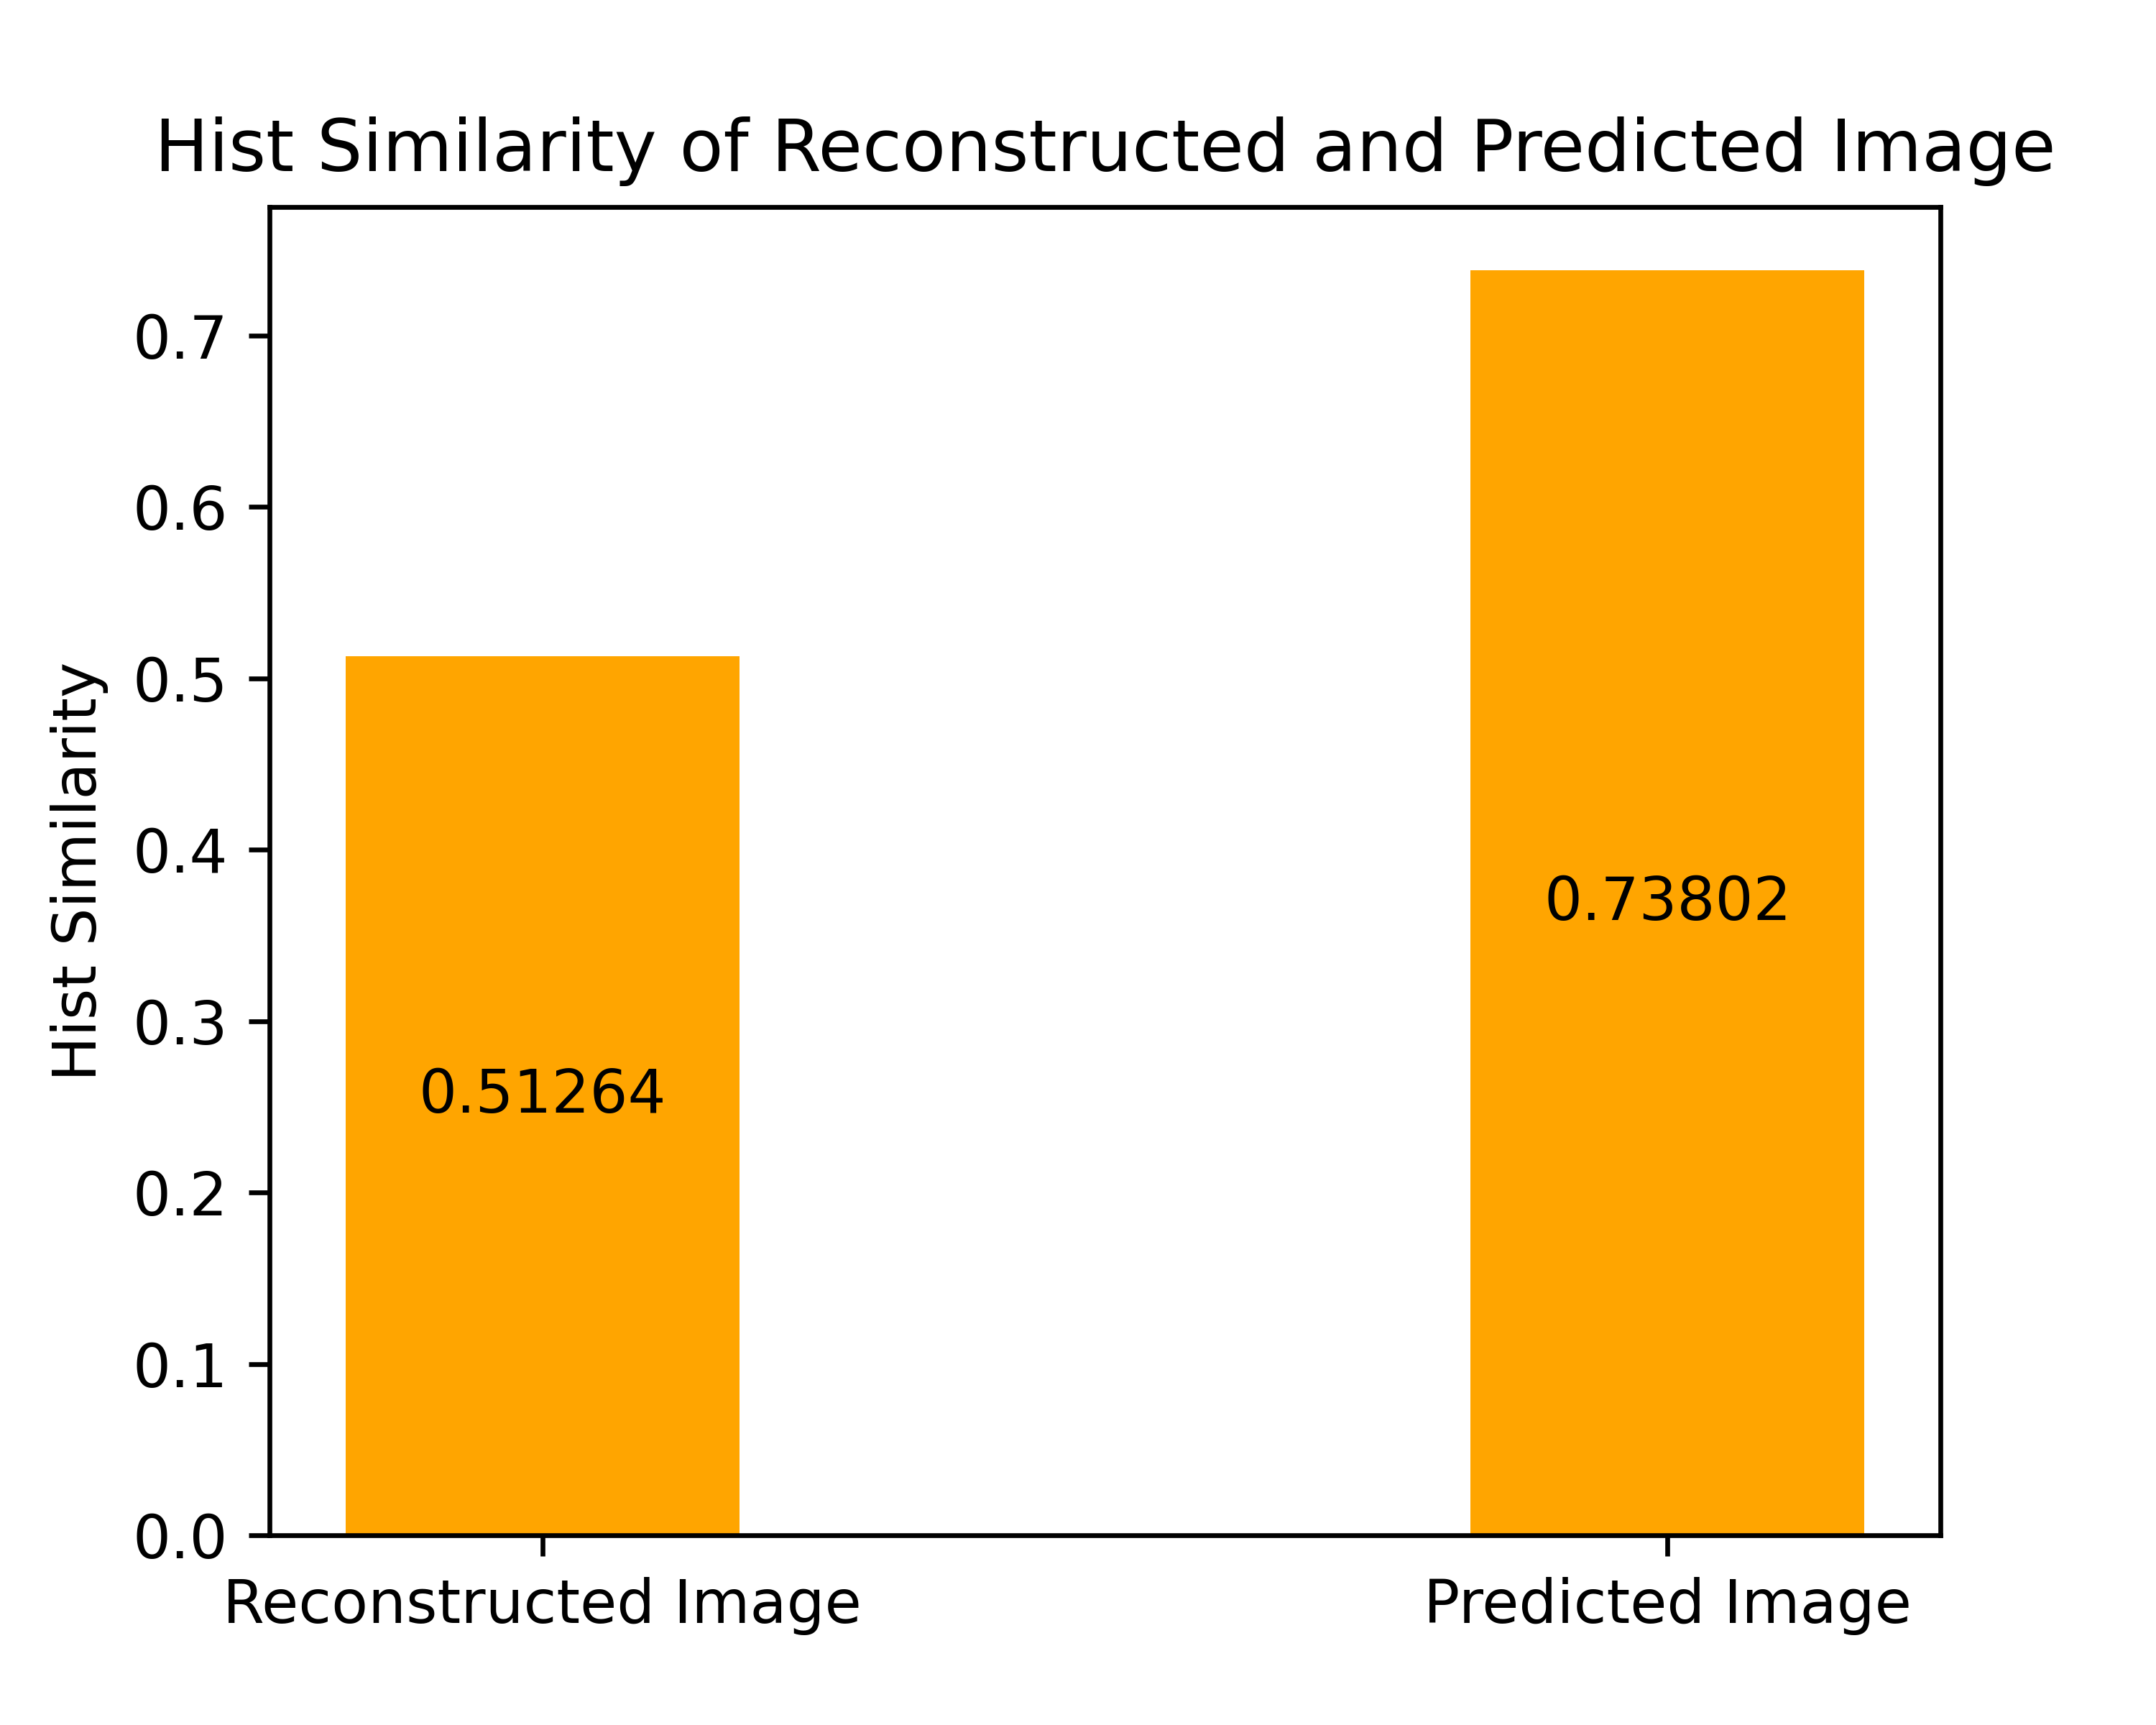
\includegraphics[width=0.75\columnwidth]{image/chap06/img610.png}
	\caption{测试集图像及其预测图象与原图像的直方图相似度的均值}
	\label{fig610}
\end{figure}

由图\ref{fig610}可知,重建图像与原图像之间的直方图相似度低于预测图像与原图像之间的直方图相似度。这说明预测图像相比于重建图像,在各像素值的统计学标准上更接近于原图像。

\section{归一化互信息}
\subsection{归一化互信息简介}
在信息论中,归一化互信息(NMI)是衡量两个随机变量之间的依赖程度大小的一项指标。NMI的值越大代表两个随机变量间的依赖程度越高。若将其运用于分析两个图片间的相似程度,则NMI的值越大代表两张图片具有越高的相似性。

对于两幅图像A与B,其归一化互信息的计算分成三步:

\begin{enumerate}
	\item 分别计算图像A,B的信息熵,其计算公式如下。
	
	\begin{equation}\label{612}
		H(A) = -\sum_aP_A(a)log_2P_A(a)
	\end{equation}

	\begin{equation}\label{613}
		H(B) = -\sum_bP_B(b)log_2P_B(b)
	\end{equation}

	其中,公式中a为图像A中的各像素值(若A为256值的灰度图像,则a的取值范围为[0,255])。像素值a的概率值$P_A(a)$为对图像进行灰度直方图统计后,像素值a所占像素点个数占全图像素点个数的比例值。对于公式(\ref{613})同理。
	
	\item 使用A与B各自的信息熵计算二者的联合信息熵。
	
	\begin{equation}\label{614}
		H(A,B)=-\sum_{a,b}P_{AB}(a,b)log_2P_{AB}(a,b)
	\end{equation}
	
	其中,公式中的a,b为图像A、B的各像素值(若A、B为256值的灰度图像,则a、b的取值范围均为[0,255]);联合概率密度$P_{AB}(a,b)$指的是两图在相同坐标系下,满足A的像素值为a且B的像素值为b的像素点,其个数占全图总像素点个数的比例值。
	
	\item 计算归一化信息熵。将第一第二步计算的A与B的信息熵H(A),H(B)及其联合信息熵H(A,B)代入如下的公式中得到归一化信息熵。
	
	\begin{equation}\label{615}
		NMI(A,B)=\cfrac{H(A)+H(B)}{H(A,B)}
	\end{equation}
\end{enumerate}

\subsection{使用互信息衡量模型效果}
对验证集的1000张图像,我们计算了原图像与重建图像或预测图像间的归一化互信息,其结果如图\ref{fig611}所示。

\begin{figure}[h]
	\centering
	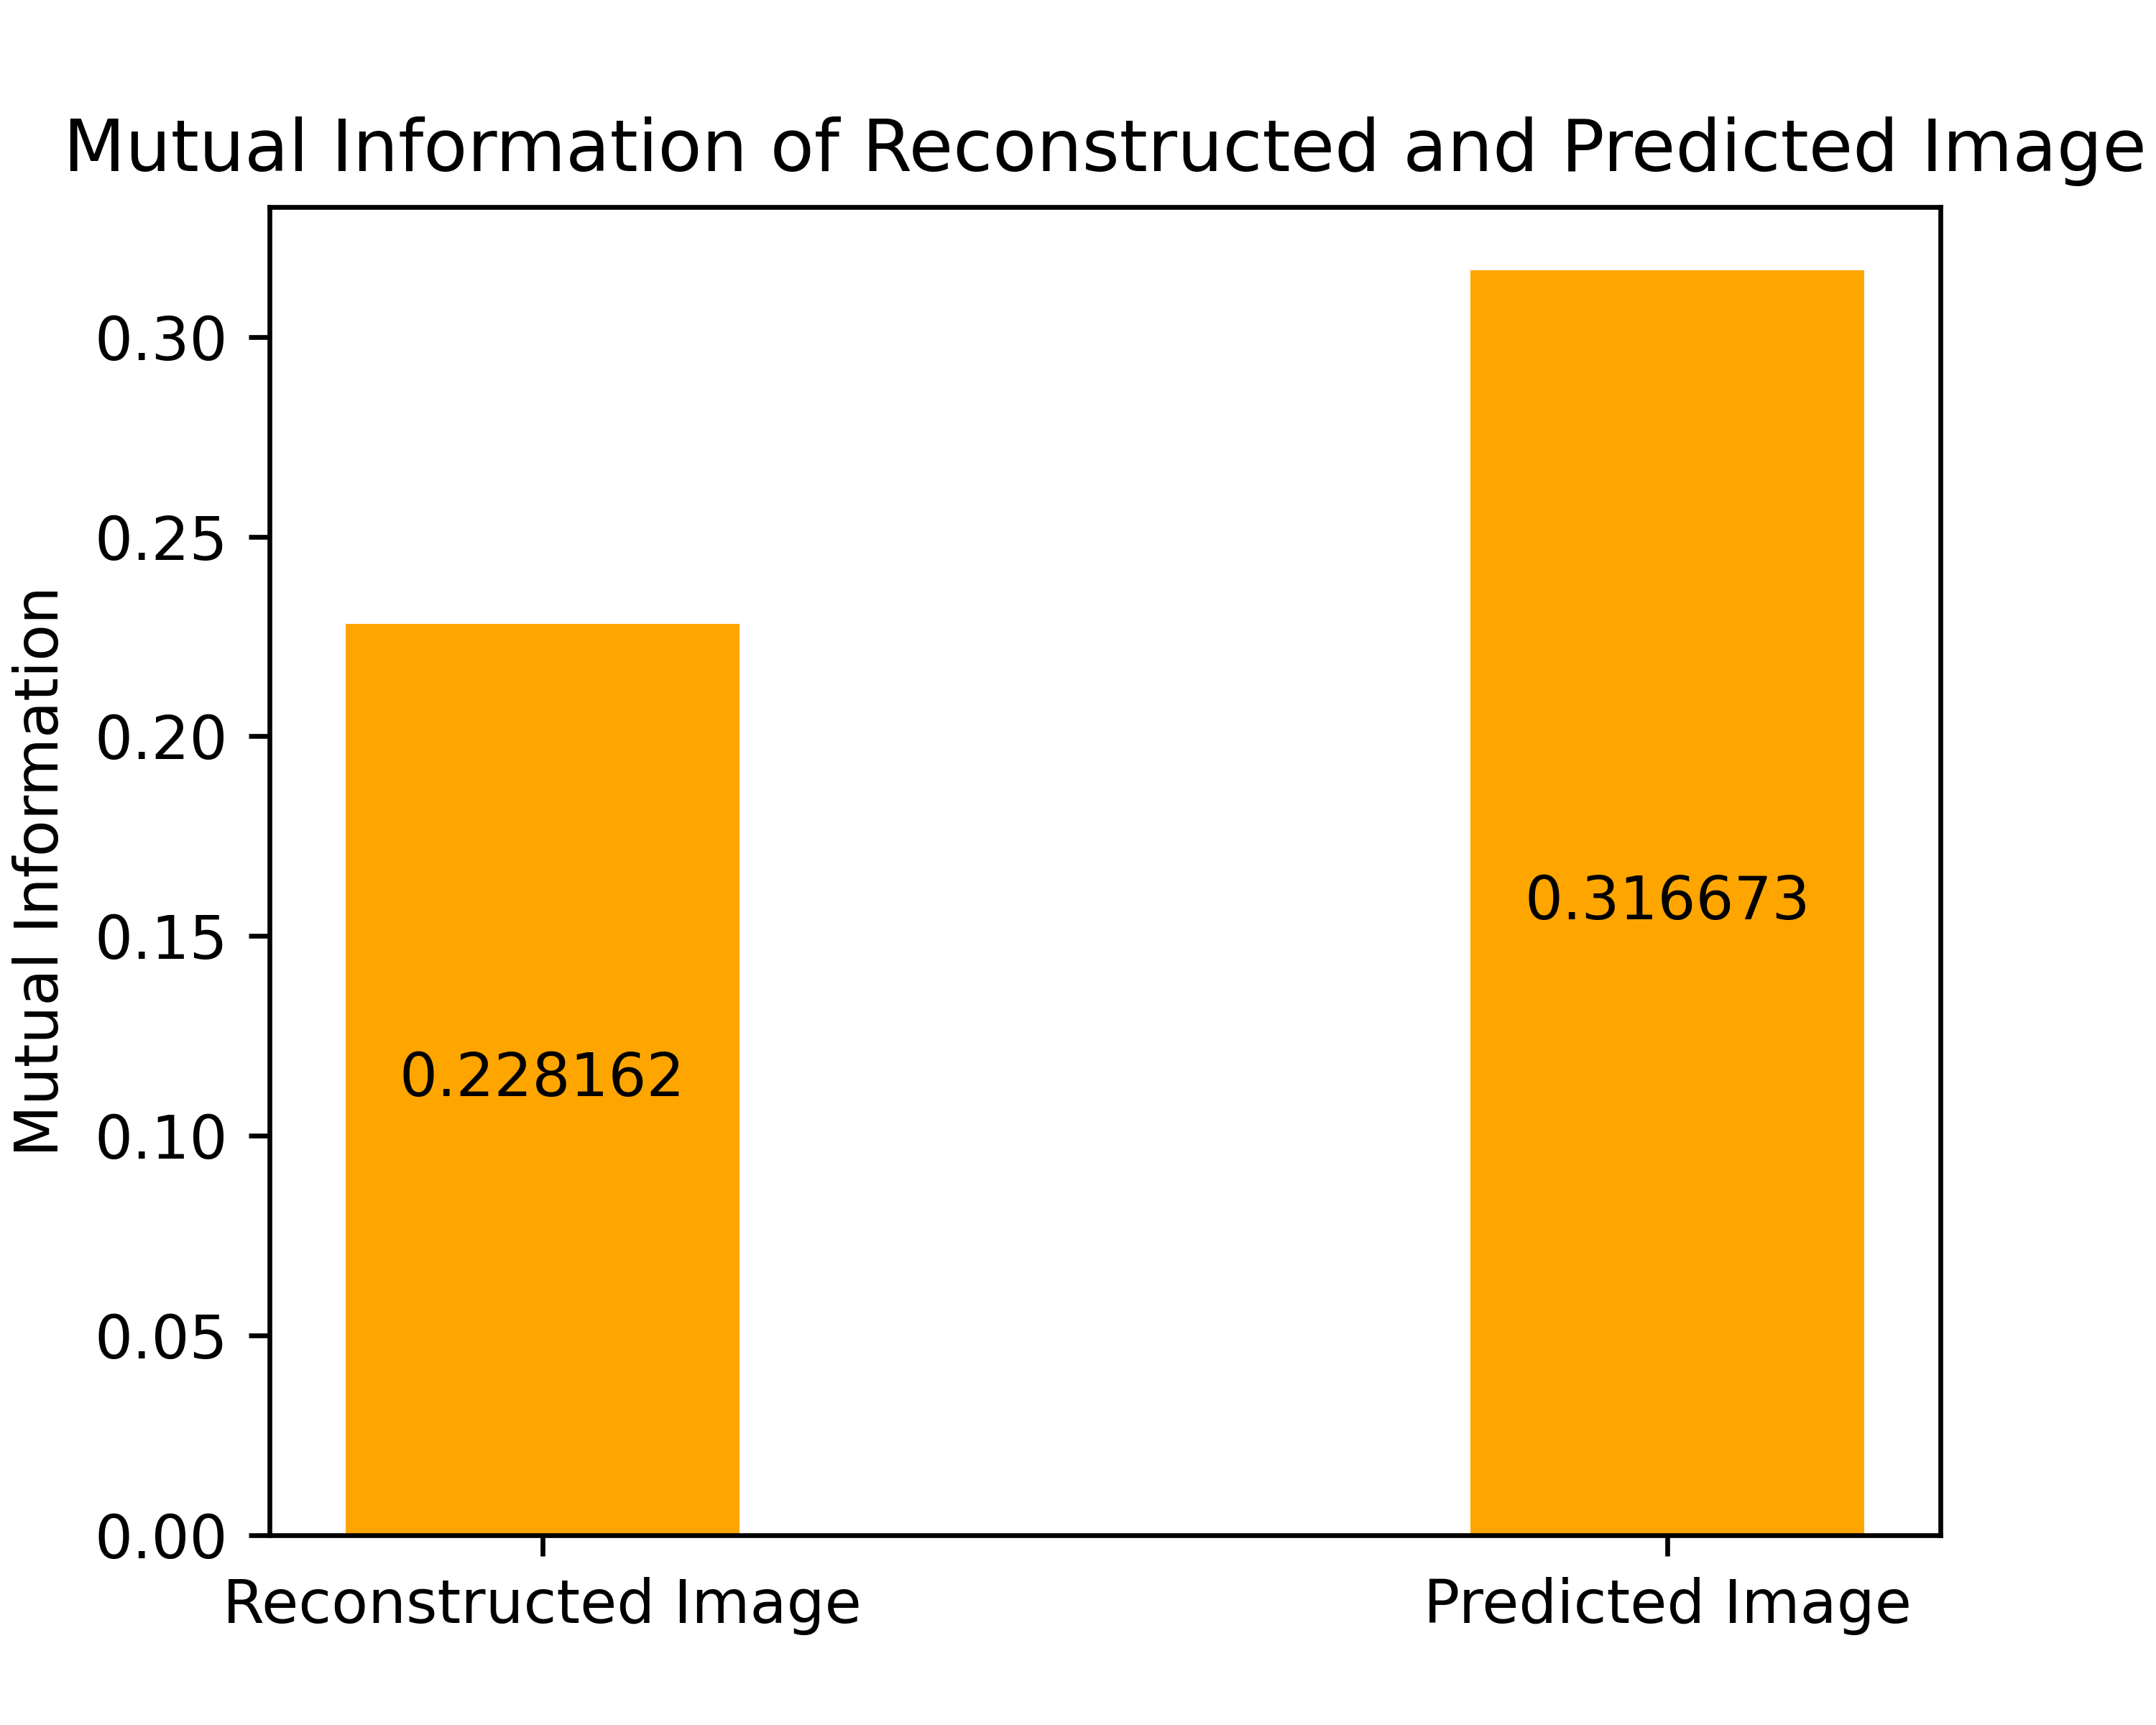
\includegraphics[width=0.75\columnwidth]{image/chap06/img611.png}
	\caption{测试集图像及其预测图象与原图像的NMI的均值}
	\label{fig611}
\end{figure}

从计算结果可知,预测图像与原图像之间的NMI值大于重建图像与原图像间的NMI值。其结果表明,预测图像比重建图像具有更高的相似性。

\section{模型评估总结}
对于验证集中的皮肤癌图片,我们计算出这1000张预测图像与原图像、重建图像与原图像的上述各评价指标的均值,记录如下表:

\begin{table}[h]
	\caption{验证集的各项评价指标的均值}
	\begin{tabular}{c|cccc}
		\hline
		& MSE                                                                                                                    & PSNR              & SSIM               & Cosine             \\ \hline
		\begin{tabular}[c]{@{}c@{}}Reconstructed\\ Image\end{tabular} & 274.263                                                                                                                & 24.6191           & 0.546436           & 0.934411           \\ \hline
		\begin{tabular}[c]{@{}c@{}}Predicted\\ Image\end{tabular}     & 126.677$\downarrow$                                                                                                    & 28.7648$\uparrow$ & 0.725969$\uparrow$ & 0.967805$\uparrow$ \\ \hline
		& Hash                                                                                                                   & Hist              & NMI                &                    \\ \hline
		\begin{tabular}[c]{@{}c@{}}Reconstructed\\ Image\end{tabular} & \begin{tabular}[c]{@{}c@{}}pHash:0.9015\\ aHash:0.911672\\ dHash:0.742875\end{tabular}                                 & 0.51264           & 0.228162           &                    \\ \hline
		\begin{tabular}[c]{@{}c@{}}Predicted\\ Image\end{tabular}     & \begin{tabular}[c]{@{}c@{}}pHash:0.949906$\uparrow$\\ aHash:0.951219$\uparrow$\\ dHash:0.842469$\uparrow$\end{tabular} & 0.73802$\uparrow$ & 0.316673$\uparrow$ &                    \\ \hline
	\end{tabular}
\end{table}


根据上述各指标的评估结果可知:训练出的神经网络模型的优化图像在逐像素比较的评估标准(MSE、PSNR、Hist)下均能取得相较重建图像更好的分辨率;且在结构相似度的评价指标SSIM下也具有更好的表现;在余弦相似度和哈希相似度等指标下也具有更高的相似度;在信息论的评价标准(NMI)下,预测图像相较于重建图像丢失更少的信息,具有更高的还原度。

因此,可以得出结论:Transformer模型在将低质量光声重建图像预测为高质量光声重建图像的优化任务上,具有较好的优化效果。将该模型应用于光声成像的后处理能显著改善采样信息丢失导致的成像精度低的问题,为低成本下获取高精度光声图像的研究提供了一个解决方法。

\section{模型不足与发展方向}
	\begin{itemize}
	\item [1)]由于项目实施的时间有限,数据集的图片数量和丰富程度还不够充实。在今后的优化中,可以适当增加数据集的来源,或通过在光声成像的仿真及重建中设置不同的传感器数量等方式来获取更丰富的数据集。
	\item [2)]由于训练次数有限,该模型在优化50个传感器下的重建图像上效果显著;而在优化100、200、400个传感器下的重建图像的效果并不是很好。这点可以通过增加由100、200、400个传感器得出的重建图像的数据集及增加训练epoch次数等方式解决。
	\item [3)]在医学的运用过程中,模型的推理成本也是一项很重要的指标。在今后的优化中,可以通过量化、剪枝\cite{rao2021dynamicvit}、知识蒸馏\cite{touvron2021training} \cite{wu2022tinyvit}、参数共享\cite{zhang2022minivit}等方法减少内存消耗与提高模型运行速度。
\end{itemize}